\begin{frame}

\end{frame}

\begin{frame}{Types of Relationships}
\protect\hypertarget{types-of-relationships}{}

\begin{enumerate}
\tightlist
\item
  Deterministic or Functional Relationship
\item
  Statistical Relationship
\end{enumerate}

\end{frame}

\begin{frame}{Deterministic Relationship}
\protect\hypertarget{deterministic-relationship}{}

Consider relationship between temperature in degrees Celsius \((C)\) and
temperature in degrees Fahrenheit \((F)\) \[F=\frac{9}{5}C+32\]
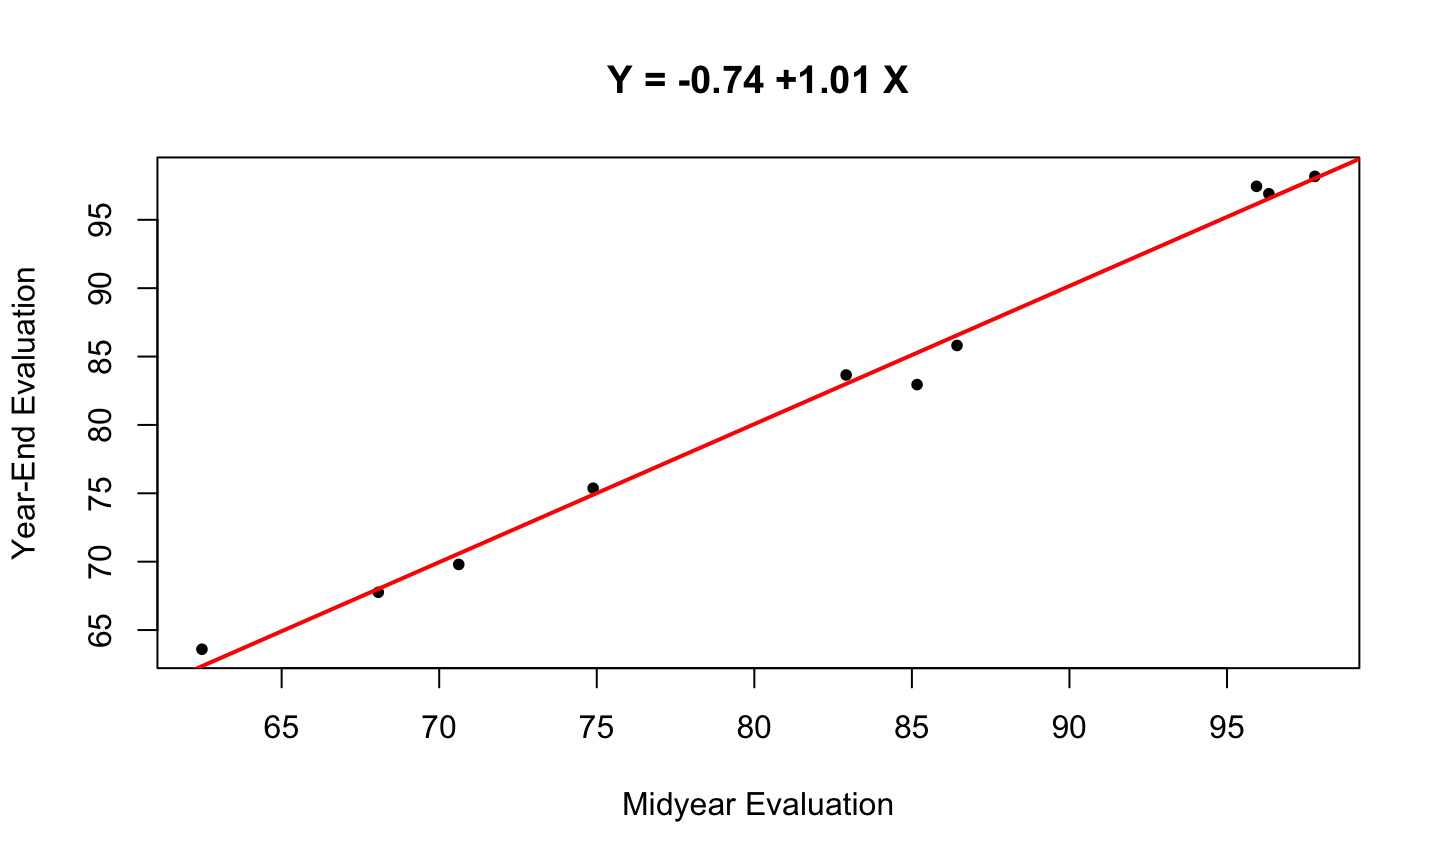
\includegraphics{chapter1_files/figure-beamer/unnamed-chunk-1-1.pdf}

\end{frame}

\begin{frame}{Statistical Relationships}
\protect\hypertarget{statistical-relationships}{}

\begin{enumerate}
\tightlist
\item
  Not an exact relationship
\item
  A relationship in which {trend} exists between \(x\) and \(y\)
  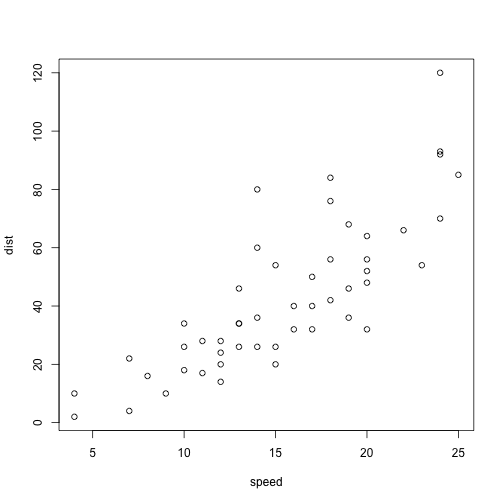
\includegraphics{chapter1_files/figure-beamer/unnamed-chunk-2-1.pdf}
\end{enumerate}

\end{frame}

\begin{frame}{Statistics analysis}
\protect\hypertarget{statistics-analysis}{}

\begin{enumerate}
\tightlist
\item
  Starts with a problem or question of interest
\item
  Proceeds with the collection of relevant data
\item
  Continues with the analysis the collected data
\item
  Ends with conclusion and interpretation of the results.
\end{enumerate}

The formulation of a problem is often more essential than its solution
which may be merely a matter of mathematical or experimental skill.
Albert Einstein

\end{frame}

\begin{frame}{Problem Formulation}
\protect\hypertarget{problem-formulation}{}

\begin{itemize}
\tightlist
\item
  Understand the physical background.

  \begin{itemize}
  \tightlist
  \item
    Statisticians often work in collaboration with others and need to
    understand something about the subject area.
  \end{itemize}
\item
  Understand the objective.

  \begin{itemize}
  \tightlist
  \item
    What are your goals?
  \item
    Make sure you know what the client wants.
  \end{itemize}
\item
  Put the problem into statistical terms.

  \begin{itemize}
  \tightlist
  \item
    This is often the most challenging step and where irreparable errors
    are sometimes made.
  \item
    That a statistical method can read in and process the data is not
    enough. The results of an inapt analysis may be meaningless.
  \end{itemize}
\end{itemize}

\end{frame}

\begin{frame}{Essentials of R}
\protect\hypertarget{essentials-of-r}{}

What is R?

\begin{itemize}
\tightlist
\item
  R is free statistical software.
\item
  R is a programming language.

  \begin{itemize}
  \tightlist
  \item
    It is an open source implementation of the S programming language.
  \item
    It is highly extendable. Users can write functions and easily add
    software libraries to R.
  \item
    It is interactive. You type what you want and get out the
    corresponding results.
  \end{itemize}
\end{itemize}

\end{frame}

\begin{frame}[fragile]{Help}
\protect\hypertarget{help}{}

There are many ways to get help for R:

\begin{itemize}
\tightlist
\item
  If you know the command you want help for, from the command line type:

  \begin{itemize}
  \tightlist
  \item
    \texttt{help(command)}

    \begin{itemize}
    \tightlist
    \item
      E.g., \texttt{help(lm)}
    \item
      \texttt{?command}
    \item
      E.g., \texttt{?lm}
    \end{itemize}
  \end{itemize}
\item
  If you only know the topic you want help for, from the command line
  type:

  \begin{itemize}
  \tightlist
  \item
    \texttt{??topic}
  \item
    E.g., \texttt{??logarithm}
  \end{itemize}
\end{itemize}

\end{frame}

\begin{frame}{Data Structure}
\protect\hypertarget{data-structure}{}

R operates on data structures. A data structure is simply some sort of
``container'' that holds certain kinds of information.

Common R data structures:

\begin{itemize}
\tightlist
\item
  Vector (a sequence of numerical, character, factor, or logical data).
\item
  Matrices (multi-dimensional collection of vectors of the same type)
\item
  Data Frame (multi-dimensional collection of possibly different data
  types)
\item
  List (an ordered collection of possibly different data types)
\end{itemize}

\end{frame}

\begin{frame}[fragile]{Vector}
\protect\hypertarget{vector}{}

A vector is a sequence of values of the same data type.

The c function (concatenate) can be used to join data from end to end to
create vectors.

\begin{itemize}
\tightlist
\item
  \texttt{c(1,\ 2,\ 5.3,\ 6,\ -2,\ 4)}
\item
  \texttt{c(“one”,\ “two”,\ “three”)}
\item
  \texttt{c(TRUE,\ TRUE,\ FALSE,\ TRUE)}
\end{itemize}

\end{frame}

\begin{frame}[fragile]{The \texttt{seq} function}
\protect\hypertarget{the-seq-function}{}

\begin{Shaded}
\begin{Highlighting}[]
\KeywordTok{seq}\NormalTok{(}\DecValTok{1}\NormalTok{,}\DecValTok{10}\NormalTok{)}
\end{Highlighting}
\end{Shaded}

\begin{verbatim}
##  [1]  1  2  3  4  5  6  7  8  9 10
\end{verbatim}

\begin{Shaded}
\begin{Highlighting}[]
\DecValTok{1}\OperatorTok{:}\DecValTok{10}
\end{Highlighting}
\end{Shaded}

\begin{verbatim}
##  [1]  1  2  3  4  5  6  7  8  9 10
\end{verbatim}

\begin{Shaded}
\begin{Highlighting}[]
\KeywordTok{seq}\NormalTok{(}\DecValTok{1}\NormalTok{, }\DecValTok{20}\NormalTok{, }\DataTypeTok{by =} \DecValTok{2}\NormalTok{)}
\end{Highlighting}
\end{Shaded}

\begin{verbatim}
##  [1]  1  3  5  7  9 11 13 15 17 19
\end{verbatim}

\begin{Shaded}
\begin{Highlighting}[]
\KeywordTok{seq}\NormalTok{(}\DecValTok{1}\NormalTok{, }\DecValTok{2}\NormalTok{, }\DataTypeTok{len =} \DecValTok{8}\NormalTok{)}
\end{Highlighting}
\end{Shaded}

\begin{verbatim}
## [1] 1.000000 1.142857 1.285714 1.428571 1.571429 1.714286 1.857143 2.000000
\end{verbatim}

\end{frame}

\begin{frame}[fragile]{The \texttt{rep} function}
\protect\hypertarget{the-rep-function}{}

The rep function (replicate) can be used to create a vector by replicate
values.

\begin{itemize}
\tightlist
\item
  Repeat the sequence 1, 2, 3 three times in a row.
\end{itemize}

\begin{Shaded}
\begin{Highlighting}[]
    \KeywordTok{rep}\NormalTok{(}\DecValTok{1}\OperatorTok{:}\DecValTok{3}\NormalTok{, }\DataTypeTok{times =} \DecValTok{3}\NormalTok{)}
\end{Highlighting}
\end{Shaded}

\begin{verbatim}
## [1] 1 2 3 1 2 3 1 2 3
\end{verbatim}

\begin{itemize}
\tightlist
\item
  Repeat ``trt1'' once, ``trt2'' twice, and ``trt3'' three times.
\end{itemize}

\begin{Shaded}
\begin{Highlighting}[]
\KeywordTok{rep}\NormalTok{(}\KeywordTok{c}\NormalTok{(}\StringTok{"trt1"}\NormalTok{, }\StringTok{"trt2"}\NormalTok{, }\StringTok{"trt3"}\NormalTok{), }\DataTypeTok{times =} \DecValTok{1}\OperatorTok{:}\DecValTok{3}\NormalTok{)}
\end{Highlighting}
\end{Shaded}

\begin{verbatim}
## [1] "trt1" "trt2" "trt2" "trt3" "trt3" "trt3"
\end{verbatim}

\begin{itemize}
\tightlist
\item
  Repeat trt1, trt2, trt3 three times each
\end{itemize}

\begin{Shaded}
\begin{Highlighting}[]
\KeywordTok{rep}\NormalTok{(}\KeywordTok{c}\NormalTok{(}\StringTok{'trt1'}\NormalTok{, }\StringTok{'trt2'}\NormalTok{, }\StringTok{"trt3"}\NormalTok{),}\DataTypeTok{each =}\DecValTok{3}\NormalTok{)}
\end{Highlighting}
\end{Shaded}

\begin{verbatim}
## [1] "trt1" "trt1" "trt1" "trt2" "trt2" "trt2" "trt3" "trt3" "trt3"
\end{verbatim}

\end{frame}

\begin{frame}[fragile]{Assignment}
\protect\hypertarget{assignment}{}

\begin{itemize}
\tightlist
\item
  To store a data structure in the computer's memory we must assign it
  to an object or name.
\item
  Data structures can be stored using the assignment operator
  ``\textless-'' or ``=''
\end{itemize}

\begin{Shaded}
\begin{Highlighting}[]
\NormalTok{    v1 <-}\StringTok{ }\DecValTok{1}\OperatorTok{:}\DecValTok{5}
\end{Highlighting}
\end{Shaded}

\begin{itemize}
\tightlist
\item
  To print the data stored in an object, we simply type the variable
  name into R and hit enter.
\end{itemize}

\begin{Shaded}
\begin{Highlighting}[]
\NormalTok{    v1}
\end{Highlighting}
\end{Shaded}

\begin{verbatim}
## [1] 1 2 3 4 5
\end{verbatim}

\begin{Shaded}
\begin{Highlighting}[]
\NormalTok{    v2 <-}\StringTok{ }\KeywordTok{c}\NormalTok{(}\DecValTok{1}\NormalTok{, }\DecValTok{10}\NormalTok{, }\DecValTok{11}\NormalTok{)}
\NormalTok{    new <-}\StringTok{ }\KeywordTok{c}\NormalTok{(v1, v2)}
\NormalTok{    new}
\end{Highlighting}
\end{Shaded}

\begin{verbatim}
## [1]  1  2  3  4  5  1 10 11
\end{verbatim}

\end{frame}

\begin{frame}[fragile]{Logical}
\protect\hypertarget{logical}{}

\begin{Shaded}
\begin{Highlighting}[]
\NormalTok{x =}\StringTok{ }\KeywordTok{seq}\NormalTok{(}\DecValTok{0}\NormalTok{,}\DecValTok{10}\NormalTok{)}
\NormalTok{x }\OperatorTok{>}\StringTok{ }\DecValTok{5}
\end{Highlighting}
\end{Shaded}

\begin{verbatim}
##  [1] FALSE FALSE FALSE FALSE FALSE FALSE  TRUE  TRUE  TRUE  TRUE  TRUE
\end{verbatim}

\begin{Shaded}
\begin{Highlighting}[]
\NormalTok{x[}\DecValTok{3}\NormalTok{]}
\end{Highlighting}
\end{Shaded}

\begin{verbatim}
## [1] 2
\end{verbatim}

\begin{Shaded}
\begin{Highlighting}[]
\NormalTok{x[}\DecValTok{3}\NormalTok{] }\OperatorTok{==}\StringTok{ }\DecValTok{2}
\end{Highlighting}
\end{Shaded}

\begin{verbatim}
## [1] TRUE
\end{verbatim}

\end{frame}

\begin{frame}[fragile]{Floating point arithmetic}
\protect\hypertarget{floating-point-arithmetic}{}

\begin{Shaded}
\begin{Highlighting}[]
\NormalTok{y =}\StringTok{ }\KeywordTok{seq}\NormalTok{(}\DecValTok{0}\NormalTok{,}\DecValTok{1}\NormalTok{,}\FloatTok{0.1}\NormalTok{)}
\NormalTok{y[}\DecValTok{5}\NormalTok{]}\OperatorTok{==}\FloatTok{0.4}
\end{Highlighting}
\end{Shaded}

\begin{verbatim}
## [1] TRUE
\end{verbatim}

\begin{Shaded}
\begin{Highlighting}[]
\NormalTok{y[}\DecValTok{9}\NormalTok{]}\OperatorTok{==}\FloatTok{0.8}
\end{Highlighting}
\end{Shaded}

\begin{verbatim}
## [1] TRUE
\end{verbatim}

\begin{Shaded}
\begin{Highlighting}[]
\NormalTok{y[}\DecValTok{4}\NormalTok{]}\OperatorTok{==}\FloatTok{0.3}
\end{Highlighting}
\end{Shaded}

\begin{verbatim}
## [1] FALSE
\end{verbatim}

\begin{Shaded}
\begin{Highlighting}[]
\NormalTok{y[}\DecValTok{4}\NormalTok{]}
\end{Highlighting}
\end{Shaded}

\begin{verbatim}
## [1] 0.3
\end{verbatim}

\begin{Shaded}
\begin{Highlighting}[]
\KeywordTok{sprintf}\NormalTok{(}\StringTok{"%.10f"}\NormalTok{,y[}\DecValTok{4}\NormalTok{])}
\end{Highlighting}
\end{Shaded}

\begin{verbatim}
## [1] "0.3000000000"
\end{verbatim}

\begin{Shaded}
\begin{Highlighting}[]
\KeywordTok{sprintf}\NormalTok{(}\StringTok{"%.20f"}\NormalTok{,y[}\DecValTok{4}\NormalTok{])}
\end{Highlighting}
\end{Shaded}

\begin{verbatim}
## [1] "0.30000000000000004441"
\end{verbatim}

\end{frame}

\begin{frame}[fragile]{Categorical data}
\protect\hypertarget{categorical-data}{}

Categorical data should be stored as a factor in R.

\begin{itemize}
\tightlist
\item
  The factor function takes vectors of any data type and converts them
  to factors.
\item
  Examples:
\end{itemize}

\begin{Shaded}
\begin{Highlighting}[]
\NormalTok{    f1 <-}\StringTok{ }\KeywordTok{factor}\NormalTok{(}\KeywordTok{rep}\NormalTok{(}\DecValTok{1}\OperatorTok{:}\DecValTok{6}\NormalTok{, }\DataTypeTok{times =} \DecValTok{3}\NormalTok{))}
\NormalTok{    f1}
\end{Highlighting}
\end{Shaded}

\begin{verbatim}
##  [1] 1 2 3 4 5 6 1 2 3 4 5 6 1 2 3 4 5 6
## Levels: 1 2 3 4 5 6
\end{verbatim}

\begin{Shaded}
\begin{Highlighting}[]
\NormalTok{    f2 <-}\StringTok{ }\KeywordTok{factor}\NormalTok{(}\KeywordTok{c}\NormalTok{(}\StringTok{"a"}\NormalTok{, }\DecValTok{7}\NormalTok{, }\StringTok{"blue"}\NormalTok{, }\StringTok{"blue"}\NormalTok{))}
\NormalTok{    f2}
\end{Highlighting}
\end{Shaded}

\begin{verbatim}
## [1] a    7    blue blue
## Levels: 7 a blue
\end{verbatim}

\end{frame}

\begin{frame}[fragile]{Commonly-used Functions}
\protect\hypertarget{commonly-used-functions}{}

\begin{Shaded}
\begin{Highlighting}[]
\NormalTok{  x <-}\StringTok{ }\KeywordTok{seq}\NormalTok{(}\DecValTok{0}\NormalTok{,}\DecValTok{10}\NormalTok{)}
    \KeywordTok{length}\NormalTok{(x) }\CommentTok{#length of x}
\end{Highlighting}
\end{Shaded}

\begin{verbatim}
## [1] 11
\end{verbatim}

\begin{Shaded}
\begin{Highlighting}[]
    \KeywordTok{sum}\NormalTok{(x) }\CommentTok{#sum elements in x}
\end{Highlighting}
\end{Shaded}

\begin{verbatim}
## [1] 55
\end{verbatim}

\begin{Shaded}
\begin{Highlighting}[]
    \KeywordTok{mean}\NormalTok{(x) }\CommentTok{#mean of elements in x}
\end{Highlighting}
\end{Shaded}

\begin{verbatim}
## [1] 5
\end{verbatim}

\begin{Shaded}
\begin{Highlighting}[]
    \KeywordTok{var}\NormalTok{(x) }\CommentTok{#sample variance of elements in x}
\end{Highlighting}
\end{Shaded}

\begin{verbatim}
## [1] 11
\end{verbatim}

\begin{Shaded}
\begin{Highlighting}[]
    \KeywordTok{sd}\NormalTok{(x) }\CommentTok{#standard deviation of elements in x}
\end{Highlighting}
\end{Shaded}

\begin{verbatim}
## [1] 3.316625
\end{verbatim}

\end{frame}

\begin{frame}[fragile]{Commonly-used Functions}
\protect\hypertarget{commonly-used-functions-1}{}

\begin{Shaded}
\begin{Highlighting}[]
\NormalTok{  x <-}\StringTok{ }\KeywordTok{seq}\NormalTok{(}\DecValTok{0}\NormalTok{,}\DecValTok{10}\NormalTok{)}
    \KeywordTok{range}\NormalTok{(x) }\CommentTok{#range of elements in x}
\end{Highlighting}
\end{Shaded}

\begin{verbatim}
## [1]  0 10
\end{verbatim}

\begin{Shaded}
\begin{Highlighting}[]
    \KeywordTok{log}\NormalTok{(x) }\CommentTok{#ln of elements in x}
\end{Highlighting}
\end{Shaded}

\begin{verbatim}
##  [1]      -Inf 0.0000000 0.6931472 1.0986123 1.3862944 1.6094379 1.7917595
##  [8] 1.9459101 2.0794415 2.1972246 2.3025851
\end{verbatim}

\begin{Shaded}
\begin{Highlighting}[]
    \KeywordTok{summary}\NormalTok{(x) }\CommentTok{#6-number summary of x}
\end{Highlighting}
\end{Shaded}

\begin{verbatim}
##    Min. 1st Qu.  Median    Mean 3rd Qu.    Max. 
##     0.0     2.5     5.0     5.0     7.5    10.0
\end{verbatim}

\end{frame}

\begin{frame}[fragile]{Functions related to statistical distributions}
\protect\hypertarget{functions-related-to-statistical-distributions}{}

Suppose that a random variable X has the ``dist'' distribution

\begin{itemize}
\tightlist
\item
  \texttt{p{[}dist{]}(q,\ \ldots{})} -- returns the cdf of X evaluated
  at q, i.e., p=Pra(X≤q).
\item
  \texttt{q{[}dist{]}(p,\ \ldots{})} -- returns the inverse cdf (or
  quantile function) of X evaluated at p, i.e.,
  \(q = \inf \{x:Pr(X\leq x)\geq p\}\)
\item
  \texttt{d{[}dist{]}(x,\ \ldots{})} -- returns the mass or density of
  \(X\) evaluated at \(x\) (depending on whether it's discrete or
  continuous).
\item
  \texttt{r{[}dist{]}(n,\ \ldots{})} -- returns an i.i.d. random sample
  of size \(n\) having the same distribution as \(X\).
\item
  \ldots{} indicates that additional arguments describing the shape of
  the distribution.
\end{itemize}

\end{frame}

\begin{frame}[fragile]{Examples}
\protect\hypertarget{examples}{}

\begin{itemize}
\item
  \texttt{pnorm(1.96,\ mean\ =\ 0,\ sd\ =\ 1)} returns the probability
  that a normal random variable with mean 0 and standard deviation 1 is
  less than or equal to 1.96.
\item
  \texttt{qunif(0.6,\ min\ =0,\ max\ =\ 1)} returns the value x such
  that \(P(X\leq x)=0.6\) for a uniform random variable on the interval
  {[}0, 1{]}.
\item
  \texttt{dbinom(2,\ size\ =\ 20,\ prob\ =\ .2)} returns the probability
  that \(Pra(X=2)\) for \(X\sim \text{Binom}(n=20,\theta=0.2)\).
\item
  \texttt{dexp(1,\ rate\ =\ 2)} returns the density of an exponential
  random variable with mean = 1/2.
\item
  \texttt{rchisq(100,\ df\ =\ 5)} returns a sample of 100 observations
  from a chi-squared random variable with 5 df.
\end{itemize}

\end{frame}

\begin{frame}[fragile]{Data Frames}
\protect\hypertarget{data-frames}{}

\begin{itemize}
\tightlist
\item
  Date frames are created by passing vectors into the
  \texttt{data.frame} function.

  \begin{itemize}
  \tightlist
  \item
    The names of the columns in the data frame are the names of the
    vectors you give the \texttt{data.frame} function.
  \end{itemize}
\end{itemize}

\begin{Shaded}
\begin{Highlighting}[]
\NormalTok{        d <-}\StringTok{ }\KeywordTok{c}\NormalTok{(}\DecValTok{1}\NormalTok{, }\DecValTok{2}\NormalTok{, }\DecValTok{3}\NormalTok{, }\DecValTok{4}\NormalTok{)}
\NormalTok{        e <-}\StringTok{ }\KeywordTok{c}\NormalTok{(}\StringTok{"red"}\NormalTok{, }\StringTok{"white"}\NormalTok{, }\StringTok{"blue"}\NormalTok{, }\OtherTok{NA}\NormalTok{)}
\NormalTok{        f <-}\StringTok{ }\KeywordTok{c}\NormalTok{(}\OtherTok{TRUE}\NormalTok{, }\OtherTok{TRUE}\NormalTok{, }\OtherTok{TRUE}\NormalTok{, }\OtherTok{FALSE}\NormalTok{)}
\NormalTok{        mydataframe <-}\StringTok{ }\KeywordTok{data.frame}\NormalTok{(d,e,f) }
\NormalTok{        mydataframe}
\end{Highlighting}
\end{Shaded}

\begin{verbatim}
##   d     e     f
## 1 1   red  TRUE
## 2 2 white  TRUE
## 3 3  blue  TRUE
## 4 4  <NA> FALSE
\end{verbatim}

\end{frame}

\begin{frame}[fragile]{Data Frames}
\protect\hypertarget{data-frames-1}{}

The columns of a data frame can be renamed using the names function on
the data frame.

\begin{Shaded}
\begin{Highlighting}[]
    \KeywordTok{names}\NormalTok{(mydataframe) <-}\StringTok{ }\KeywordTok{c}\NormalTok{(}\StringTok{"ID"}\NormalTok{, }\StringTok{"Color"}\NormalTok{, }\StringTok{"Passed"}\NormalTok{)}
\NormalTok{    mydataframe}
\end{Highlighting}
\end{Shaded}

\begin{verbatim}
##   ID Color Passed
## 1  1   red   TRUE
## 2  2 white   TRUE
## 3  3  blue   TRUE
## 4  4  <NA>  FALSE
\end{verbatim}

The columns of a data frame can be named when you are first creating the
data frame by using ``name ='' for each vector of data.

\begin{Shaded}
\begin{Highlighting}[]
\NormalTok{    dataframe2 <-}\StringTok{ }\KeywordTok{data.frame}\NormalTok{(}\DataTypeTok{ID=}\NormalTok{d, }\DataTypeTok{Color=}\NormalTok{e, }\DataTypeTok{Passed=}\NormalTok{f)}
\NormalTok{    dataframe2}
\end{Highlighting}
\end{Shaded}

\begin{verbatim}
##   ID Color Passed
## 1  1   red   TRUE
## 2  2 white   TRUE
## 3  3  blue   TRUE
## 4  4  <NA>  FALSE
\end{verbatim}

\end{frame}

\begin{frame}[fragile]{Data Frames}
\protect\hypertarget{data-frames-2}{}

The vectors of a data frame may be accessed using ``\$'' and specifying
the name of the desired vector.

\begin{Shaded}
\begin{Highlighting}[]
\NormalTok{    mydataframe}\OperatorTok{$}\NormalTok{Color}
\end{Highlighting}
\end{Shaded}

\begin{verbatim}
## [1] "red"   "white" "blue"  NA
\end{verbatim}

The vectors of a data frame may be accessed by specifying the desired
row(s) or column(s) in square brackets.

\begin{Shaded}
\begin{Highlighting}[]
\NormalTok{    mydataframe[}\DecValTok{1}\NormalTok{,]}
\end{Highlighting}
\end{Shaded}

\begin{verbatim}
##   ID Color Passed
## 1  1   red   TRUE
\end{verbatim}

\begin{Shaded}
\begin{Highlighting}[]
\NormalTok{  mydataframe[,}\DecValTok{3}\NormalTok{]}
\end{Highlighting}
\end{Shaded}

\begin{verbatim}
## [1]  TRUE  TRUE  TRUE FALSE
\end{verbatim}

\end{frame}

\begin{frame}[fragile]{Data Frames}
\protect\hypertarget{data-frames-3}{}

Access the ID column of dataframe2 and assign it to newID

\begin{Shaded}
\begin{Highlighting}[]
\NormalTok{    newID <-}\StringTok{ }\NormalTok{dataframe2}\OperatorTok{$}\NormalTok{ID}
\end{Highlighting}
\end{Shaded}

Create a new ID column within the dataframe2

\begin{Shaded}
\begin{Highlighting}[]
\NormalTok{  dataframe2}\OperatorTok{$}\NormalTok{ID_new <-}\StringTok{ }\KeywordTok{paste}\NormalTok{(}\StringTok{'Bird_'}\NormalTok{,dataframe2}\OperatorTok{$}\NormalTok{ID,}\DataTypeTok{sep =} \StringTok{''}\NormalTok{)}
\NormalTok{dataframe2}
\end{Highlighting}
\end{Shaded}

\begin{verbatim}
##   ID Color Passed ID_new
## 1  1   red   TRUE Bird_1
## 2  2 white   TRUE Bird_2
## 3  3  blue   TRUE Bird_3
## 4  4  <NA>  FALSE Bird_4
\end{verbatim}

\end{frame}

\begin{frame}[fragile]{Importing Data}
\protect\hypertarget{importing-data}{}

\begin{itemize}
\tightlist
\item
  The read.table function imports data into R as a data frame.
\item
  Usage: \texttt{read.table(file,\ header\ =\ TRUE,\ sep\ =\ ",")}
\item
  file is the file path and name of the file you want to import into R

  \begin{itemize}
  \tightlist
  \item
    If you don't know the file path, set \texttt{file\ =\ file.choose()}
    will bring up a dialog box asking you to locate the file you want to
    import.
  \end{itemize}
\end{itemize}

\end{frame}

\begin{frame}[fragile]{\texttt{header} option}
\protect\hypertarget{header-option}{}

\begin{itemize}
\tightlist
\item
  \texttt{header} specifies whether the data file has a header (labels
  for each column of data in the first row of the data file).

  \begin{itemize}
  \tightlist
  \item
    If you don't specify this option in R or use \texttt{header=FALSE},
    then R will assume the file doesn't have any headings.
  \item
    \texttt{header=TRUE} tells R to read in the data as a data frame
    with column names taken from the first row of the data file.
  \end{itemize}
\end{itemize}

\end{frame}

\begin{frame}[fragile]{\texttt{sep} option}
\protect\hypertarget{sep-option}{}

\begin{itemize}
\tightlist
\item
  \texttt{sep} specifies the delimiter separating elements in the file.

  \begin{itemize}
  \tightlist
  \item
    If each column of data in the file is separated by a space, then use
    \texttt{sep\ =\ "\ "}
  \item
    If each column of data in the file is separated by a comma, then use
    \texttt{sep\ =\ ","}
  \item
    If each column of data in the file is separated by a tab, then use
    \texttt{sep\ =\ "\textbackslash{}t"}.
  \end{itemize}
\end{itemize}

Note that the \texttt{read\_table} function in the \texttt{readr}
package and the \texttt{fread} function in the \texttt{data.table}
package are perhaps better ways of reading in tabular data and use
similar syntax.

\end{frame}

\begin{frame}[fragile]{Accessing Elements of a Data Structure}
\protect\hypertarget{accessing-elements-of-a-data-structure}{}

\begin{itemize}
\item
  Subsets of the elements of a vector may be selected by appending to
  the name of the vector an index vector in square brackets.
\item
\end{itemize}

\begin{Shaded}
\begin{Highlighting}[]
\NormalTok{    a <-}\StringTok{ }\KeywordTok{seq}\NormalTok{(}\DecValTok{2}\NormalTok{, }\DecValTok{16}\NormalTok{, }\DataTypeTok{by =} \DecValTok{2}\NormalTok{)}
\NormalTok{    a}
\end{Highlighting}
\end{Shaded}

\begin{verbatim}
## [1]  2  4  6  8 10 12 14 16
\end{verbatim}

\begin{Shaded}
\begin{Highlighting}[]
\NormalTok{    a[}\KeywordTok{c}\NormalTok{(}\DecValTok{2}\NormalTok{, }\DecValTok{4}\NormalTok{, }\DecValTok{6}\NormalTok{)] }\CommentTok{#Access the 2nd, 4th, and 6th elements of a.}
\end{Highlighting}
\end{Shaded}

\begin{verbatim}
## [1]  4  8 12
\end{verbatim}

\begin{Shaded}
\begin{Highlighting}[]
\NormalTok{    a[}\OperatorTok{-}\KeywordTok{c}\NormalTok{(}\DecValTok{2}\NormalTok{, }\DecValTok{4}\NormalTok{, }\DecValTok{6}\NormalTok{)] }\CommentTok{#Access all elements in a EXCEPT the 2nd, 4th, and 6th.}
\end{Highlighting}
\end{Shaded}

\begin{verbatim}
## [1]  2  6 10 14 16
\end{verbatim}

\begin{Shaded}
\begin{Highlighting}[]
\NormalTok{    a[}\OperatorTok{-}\NormalTok{(}\DecValTok{3}\OperatorTok{:}\DecValTok{6}\NormalTok{)] }\CommentTok{#Access all elements in a except elements 3 through 6.}
\end{Highlighting}
\end{Shaded}

\begin{verbatim}
## [1]  2  4 14 16
\end{verbatim}

\end{frame}

\begin{frame}[fragile]{Logical operations}
\protect\hypertarget{logical-operations}{}

Sometimes we need to know if the elements of an object satisfy certain
conditions. This can be determined using the logical operators
\textless, \textless=, \textgreater, \textgreater=, ==, !=

\begin{itemize}
\tightlist
\item
  ``=='' means ``equal to'' and ``!='' means not equal to.
\end{itemize}

\begin{Shaded}
\begin{Highlighting}[]
\NormalTok{a <-}\StringTok{ }\KeywordTok{sample}\NormalTok{(}\DecValTok{0}\OperatorTok{:}\DecValTok{99}\NormalTok{,}\DecValTok{10}\NormalTok{)}
\NormalTok{a}
\end{Highlighting}
\end{Shaded}

\begin{verbatim}
##  [1] 59 46 64 63 43 41 80 66 20 39
\end{verbatim}

\begin{Shaded}
\begin{Highlighting}[]
\NormalTok{a}\OperatorTok{>}\DecValTok{50} 
\end{Highlighting}
\end{Shaded}

\begin{verbatim}
##  [1]  TRUE FALSE  TRUE  TRUE FALSE FALSE  TRUE  TRUE FALSE FALSE
\end{verbatim}

\begin{Shaded}
\begin{Highlighting}[]
\NormalTok{a[a}\OperatorTok{>}\DecValTok{50}\NormalTok{] }\CommentTok{#values of a greater than 50}
\end{Highlighting}
\end{Shaded}

\begin{verbatim}
## [1] 59 64 63 80 66
\end{verbatim}

\begin{Shaded}
\begin{Highlighting}[]
\NormalTok{a[a}\OperatorTok{<=}\DecValTok{40}\NormalTok{] }\CommentTok{#values of a less than or equal to 40}
\end{Highlighting}
\end{Shaded}

\begin{verbatim}
## [1] 20 39
\end{verbatim}

\end{frame}

\begin{frame}[fragile]{Logical operations}
\protect\hypertarget{logical-operations-1}{}

\begin{Shaded}
\begin{Highlighting}[]
\NormalTok{a}\OperatorTok{==}\DecValTok{10} \CommentTok{#Is there 10?}
\end{Highlighting}
\end{Shaded}

\begin{verbatim}
##  [1] FALSE FALSE FALSE FALSE FALSE FALSE FALSE FALSE FALSE FALSE
\end{verbatim}

\begin{Shaded}
\begin{Highlighting}[]
\KeywordTok{sum}\NormalTok{(a}\OperatorTok{==}\DecValTok{10}\NormalTok{)}
\end{Highlighting}
\end{Shaded}

\begin{verbatim}
## [1] 0
\end{verbatim}

\begin{Shaded}
\begin{Highlighting}[]
\DecValTok{10}\OperatorTok\NormalTok{a}
\end{Highlighting}
\end{Shaded}

\begin{verbatim}
## [1] FALSE
\end{verbatim}

\end{frame}

\begin{frame}[fragile]{Logical operations}
\protect\hypertarget{logical-operations-2}{}

\begin{itemize}
\tightlist
\item
  More complicated logical arguments can be made using \texttt{\&} and
  \texttt{\textbar{}}.

  \begin{itemize}
  \item
    \& means ``and''
  \item
    means ``or''
  \end{itemize}
\end{itemize}

\begin{Shaded}
\begin{Highlighting}[]
\NormalTok{(a }\OperatorTok{>}\StringTok{ }\DecValTok{50}\NormalTok{) }\OperatorTok{&}\StringTok{ }\NormalTok{(a }\OperatorTok{<=}\StringTok{ }\DecValTok{90}\NormalTok{) }\CommentTok{#Elements of a greater than 50 and less than or equal to 90}
\end{Highlighting}
\end{Shaded}

\begin{verbatim}
##  [1]  TRUE FALSE  TRUE  TRUE FALSE FALSE  TRUE  TRUE FALSE FALSE
\end{verbatim}

\begin{Shaded}
\begin{Highlighting}[]
\NormalTok{a[(a }\OperatorTok{>}\StringTok{ }\DecValTok{50}\NormalTok{) }\OperatorTok{&}\StringTok{ }\NormalTok{(a }\OperatorTok{<=}\StringTok{ }\DecValTok{90}\NormalTok{)]}
\end{Highlighting}
\end{Shaded}

\begin{verbatim}
## [1] 59 64 63 80 66
\end{verbatim}

\begin{Shaded}
\begin{Highlighting}[]
\NormalTok{a[(a }\OperatorTok{<=}\StringTok{ }\DecValTok{30}\NormalTok{) }\OperatorTok{|}\StringTok{ }\NormalTok{(a}\OperatorTok{>=}\DecValTok{70}\NormalTok{)]}
\end{Highlighting}
\end{Shaded}

\begin{verbatim}
## [1] 80 20
\end{verbatim}

\end{frame}

\begin{frame}[fragile]{Other data management options}
\protect\hypertarget{other-data-management-options}{}

Note: There is now a debate about the proper approach to organizing and
working with data.

We will typically work with base R.

\begin{itemize}
\tightlist
\item
  These are the commands and functions R offers by default.
\end{itemize}

The \texttt{tidyverse} (www.tidyverse.org) is a collection of R packages
that provides a unified framework for data manipulation and
visualization.

\begin{itemize}
\tightlist
\item
  This is becoming extremely popular.
\item
  Since this course is focuses more on modeling than data manipulation
  (though we will have to do this), I will typically only use functions
  from the tidyverse when it greatly simplifies analysis, data
  manipulation, or visualization.
\end{itemize}

\end{frame}

\begin{frame}{Sample Data Analysis in R}
\protect\hypertarget{sample-data-analysis-in-r}{}

Calculate numerical summaries:

\begin{itemize}
\tightlist
\item
  means
\item
  standard deviations (SDs)
\item
  maximum and minimum, correlations
\item
  anything else that may be appropriate.
\end{itemize}

Construct the appropriate plots.

\begin{itemize}
\tightlist
\item
  For one quantitative variable: boxplots, histograms, density plots,
  etc.
\item
  For two quantitative variables: scatterplots.
\item
  For three or more variables, construct interactive and dynamic
  graphics.
\end{itemize}

\end{frame}

\begin{frame}{Kidney Example}
\protect\hypertarget{kidney-example}{}

The National Institute of Diabetes and Digestive and Kidney Diseases
conducted a study on 768 adult female Pima Indians living near Phoenix.
The following variables were recorded: number of times pregnant, plasma
glucose concentration at 2 hours in an oral glucose tolerance test,
diastolic blood pressure (mmHg), triceps skin fold thickness (mm),
2-hour serum insulin (mu U/ml), body mass index (weight in kg/(height in
m2)), diabetes pedigree function, age (years) and a test whether the
patient showed signs of diabetes (coded zero if negative, one if
positive). The data may be obtained from the UCI Repository of machine
learning databases at archive.ics.uci.edu/ml.

\end{frame}

\begin{frame}[fragile]{Load data}
\protect\hypertarget{load-data}{}

\begin{Shaded}
\begin{Highlighting}[]
\KeywordTok{data}\NormalTok{(pima, }\DataTypeTok{package =} \StringTok{"faraway"}\NormalTok{)}
\KeywordTok{str}\NormalTok{(pima)}
\end{Highlighting}
\end{Shaded}

\begin{verbatim}
## 'data.frame':    768 obs. of  9 variables:
##  $ pregnant : int  6 1 8 1 0 5 3 10 2 8 ...
##  $ glucose  : int  148 85 183 89 137 116 78 115 197 125 ...
##  $ diastolic: int  72 66 64 66 40 74 50 0 70 96 ...
##  $ triceps  : int  35 29 0 23 35 0 32 0 45 0 ...
##  $ insulin  : int  0 0 0 94 168 0 88 0 543 0 ...
##  $ bmi      : num  33.6 26.6 23.3 28.1 43.1 25.6 31 35.3 30.5 0 ...
##  $ diabetes : num  0.627 0.351 0.672 0.167 2.288 ...
##  $ age      : int  50 31 32 21 33 30 26 29 53 54 ...
##  $ test     : int  1 0 1 0 1 0 1 0 1 1 ...
\end{verbatim}

\end{frame}

\begin{frame}[fragile]{Data head and tail}
\protect\hypertarget{data-head-and-tail}{}

\begin{Shaded}
\begin{Highlighting}[]
\KeywordTok{head}\NormalTok{(pima)}
\end{Highlighting}
\end{Shaded}

\begin{verbatim}
##   pregnant glucose diastolic triceps insulin  bmi diabetes age test
## 1        6     148        72      35       0 33.6    0.627  50    1
## 2        1      85        66      29       0 26.6    0.351  31    0
## 3        8     183        64       0       0 23.3    0.672  32    1
## 4        1      89        66      23      94 28.1    0.167  21    0
## 5        0     137        40      35     168 43.1    2.288  33    1
## 6        5     116        74       0       0 25.6    0.201  30    0
\end{verbatim}

\begin{Shaded}
\begin{Highlighting}[]
\KeywordTok{tail}\NormalTok{(pima)}
\end{Highlighting}
\end{Shaded}

\begin{verbatim}
##     pregnant glucose diastolic triceps insulin  bmi diabetes age test
## 763        9      89        62       0       0 22.5    0.142  33    0
## 764       10     101        76      48     180 32.9    0.171  63    0
## 765        2     122        70      27       0 36.8    0.340  27    0
## 766        5     121        72      23     112 26.2    0.245  30    0
## 767        1     126        60       0       0 30.1    0.349  47    1
## 768        1      93        70      31       0 30.4    0.315  23    0
\end{verbatim}

\end{frame}

\begin{frame}[fragile]{Data entry errors}
\protect\hypertarget{data-entry-errors}{}

The \texttt{summary} command is a quick way to get the usual univariate
summary information.

\begin{itemize}
\tightlist
\item
  Look for anything unusual or unexpected, perhaps indicating a
  data-entry error.
\item
  The minimum blood pressure is zero! (That's generally an indication of
  a problem).
\end{itemize}

\begin{Shaded}
\begin{Highlighting}[]
\KeywordTok{sort}\NormalTok{(pima}\OperatorTok{$}\NormalTok{diastolic)}
\end{Highlighting}
\end{Shaded}

\begin{verbatim}
##   [1]   0   0   0   0   0   0   0   0   0   0   0   0   0   0   0   0   0   0
##  [19]   0   0   0   0   0   0   0   0   0   0   0   0   0   0   0   0   0  24
##  [37]  30  30  38  40  44  44  44  44  46  46  48  48  48  48  48  50  50  50
##  [55]  50  50  50  50  50  50  50  50  50  50  52  52  52  52  52  52  52  52
##  [73]  52  52  52  54  54  54  54  54  54  54  54  54  54  54  55  55  56  56
##  [91]  56  56  56  56  56  56  56  56  56  56  58  58  58  58  58  58  58  58
## [109]  58  58  58  58  58  58  58  58  58  58  58  58  58  60  60  60  60  60
## [127]  60  60  60  60  60  60  60  60  60  60  60  60  60  60  60  60  60  60
## [145]  60  60  60  60  60  60  60  60  60  60  60  60  60  60  61  62  62  62
## [163]  62  62  62  62  62  62  62  62  62  62  62  62  62  62  62  62  62  62
## [181]  62  62  62  62  62  62  62  62  62  62  62  62  62  64  64  64  64  64
## [199]  64  64  64  64  64  64  64  64  64  64  64  64  64  64  64  64  64  64
## [217]  64  64  64  64  64  64  64  64  64  64  64  64  64  64  64  64  64  64
## [235]  64  64  65  65  65  65  65  65  65  66  66  66  66  66  66  66  66  66
## [253]  66  66  66  66  66  66  66  66  66  66  66  66  66  66  66  66  66  66
## [271]  66  66  66  68  68  68  68  68  68  68  68  68  68  68  68  68  68  68
## [289]  68  68  68  68  68  68  68  68  68  68  68  68  68  68  68  68  68  68
## [307]  68  68  68  68  68  68  68  68  68  68  68  68  70  70  70  70  70  70
## [325]  70  70  70  70  70  70  70  70  70  70  70  70  70  70  70  70  70  70
## [343]  70  70  70  70  70  70  70  70  70  70  70  70  70  70  70  70  70  70
## [361]  70  70  70  70  70  70  70  70  70  70  70  70  70  70  70  72  72  72
## [379]  72  72  72  72  72  72  72  72  72  72  72  72  72  72  72  72  72  72
## [397]  72  72  72  72  72  72  72  72  72  72  72  72  72  72  72  72  72  72
## [415]  72  72  72  72  72  74  74  74  74  74  74  74  74  74  74  74  74  74
## [433]  74  74  74  74  74  74  74  74  74  74  74  74  74  74  74  74  74  74
## [451]  74  74  74  74  74  74  74  74  74  74  74  74  74  74  74  74  74  74
## [469]  74  74  74  75  75  75  75  75  75  75  75  76  76  76  76  76  76  76
## [487]  76  76  76  76  76  76  76  76  76  76  76  76  76  76  76  76  76  76
## [505]  76  76  76  76  76  76  76  76  76  76  76  76  76  76  78  78  78  78
## [523]  78  78  78  78  78  78  78  78  78  78  78  78  78  78  78  78  78  78
## [541]  78  78  78  78  78  78  78  78  78  78  78  78  78  78  78  78  78  78
## [559]  78  78  78  78  78  80  80  80  80  80  80  80  80  80  80  80  80  80
## [577]  80  80  80  80  80  80  80  80  80  80  80  80  80  80  80  80  80  80
## [595]  80  80  80  80  80  80  80  80  80  82  82  82  82  82  82  82  82  82
## [613]  82  82  82  82  82  82  82  82  82  82  82  82  82  82  82  82  82  82
## [631]  82  82  82  84  84  84  84  84  84  84  84  84  84  84  84  84  84  84
## [649]  84  84  84  84  84  84  84  84  85  85  85  85  85  85  86  86  86  86
## [667]  86  86  86  86  86  86  86  86  86  86  86  86  86  86  86  86  86  88
## [685]  88  88  88  88  88  88  88  88  88  88  88  88  88  88  88  88  88  88
## [703]  88  88  88  88  88  88  90  90  90  90  90  90  90  90  90  90  90  90
## [721]  90  90  90  90  90  90  90  90  90  90  92  92  92  92  92  92  92  92
## [739]  94  94  94  94  94  94  95  96  96  96  96  98  98  98 100 100 100 102
## [757] 104 104 106 106 106 108 108 110 110 110 114 122
\end{verbatim}

\end{frame}

\begin{frame}{Data entry errors}
\protect\hypertarget{data-entry-errors-1}{}

The first 35 values are zero---there's a problem.

\begin{itemize}
\tightlist
\item
  It seems that 0 was used in place of a missing value.
\item
  This is very bad since 0 is a real number and this problem may be
  overlooked, which can lead to faulty analysis!
\item
  This is why we must check our data carefully for things that don't
  make sense.
\end{itemize}

\end{frame}

\begin{frame}[fragile]{Assing \texttt{NA} for missing data}
\protect\hypertarget{assing-na-for-missing-data}{}

The value for missing data in R is \texttt{NA}.

Several variables share this problem. Let's set the 0s that should be
missing values to \texttt{NA}.

\begin{Shaded}
\begin{Highlighting}[]
\NormalTok{pima}\OperatorTok{$}\NormalTok{diastolic[pima}\OperatorTok{$}\NormalTok{diastolic }\OperatorTok{==}\StringTok{ }\DecValTok{0}\NormalTok{]  <-}\StringTok{ }\OtherTok{NA}
\NormalTok{pima}\OperatorTok{$}\NormalTok{glucose[pima}\OperatorTok{$}\NormalTok{glucose }\OperatorTok{==}\StringTok{ }\DecValTok{0}\NormalTok{] <-}\StringTok{ }\OtherTok{NA}
\NormalTok{pima}\OperatorTok{$}\NormalTok{triceps[pima}\OperatorTok{$}\NormalTok{triceps }\OperatorTok{==}\StringTok{ }\DecValTok{0}\NormalTok{]  <-}\StringTok{ }\OtherTok{NA}
\NormalTok{pima}\OperatorTok{$}\NormalTok{insulin[pima}\OperatorTok{$}\NormalTok{insulin }\OperatorTok{==}\StringTok{ }\DecValTok{0}\NormalTok{] <-}\StringTok{ }\OtherTok{NA}
\NormalTok{pima}\OperatorTok{$}\NormalTok{bmi[pima}\OperatorTok{$}\NormalTok{bmi }\OperatorTok{==}\StringTok{ }\DecValTok{0}\NormalTok{] <-}\StringTok{ }\OtherTok{NA}
\end{Highlighting}
\end{Shaded}

\end{frame}

\begin{frame}[fragile]{Data class}
\protect\hypertarget{data-class}{}

The variable test is a categorical variable, not numerical.

\begin{itemize}
\tightlist
\item
  R thinks it is numerical.
\item
  In R, a categorical variable is a factor.
\item
  We need to convert this variable to a factor.
\end{itemize}

\begin{Shaded}
\begin{Highlighting}[]
\NormalTok{ pima}\OperatorTok{$}\NormalTok{test <-}\StringTok{ }\KeywordTok{factor}\NormalTok{(pima}\OperatorTok{$}\NormalTok{test)}
 \KeywordTok{summary}\NormalTok{(pima}\OperatorTok{$}\NormalTok{test)}
\end{Highlighting}
\end{Shaded}

\begin{verbatim}
##   0   1 
## 500 268
\end{verbatim}

500 of the cases were negative and 268 were positive. We can provide
more descriptive labels using the levels function.

\begin{Shaded}
\begin{Highlighting}[]
\KeywordTok{levels}\NormalTok{(pima}\OperatorTok{$}\NormalTok{test) <-}\KeywordTok{c}\NormalTok{(}\StringTok{"negative"}\NormalTok{,}\StringTok{"positive"}\NormalTok{)}
\end{Highlighting}
\end{Shaded}

\end{frame}

\begin{frame}[fragile]{Ploting Data}
\protect\hypertarget{ploting-data}{}

A histogram of diastolic blood pressure.

\begin{Shaded}
\begin{Highlighting}[]
\KeywordTok{hist}\NormalTok{(pima}\OperatorTok{$}\NormalTok{dias,}\DataTypeTok{xlab=}\StringTok{"Diastolic"}\NormalTok{,}\DataTypeTok{main=}\StringTok{""}\NormalTok{)}
\end{Highlighting}
\end{Shaded}

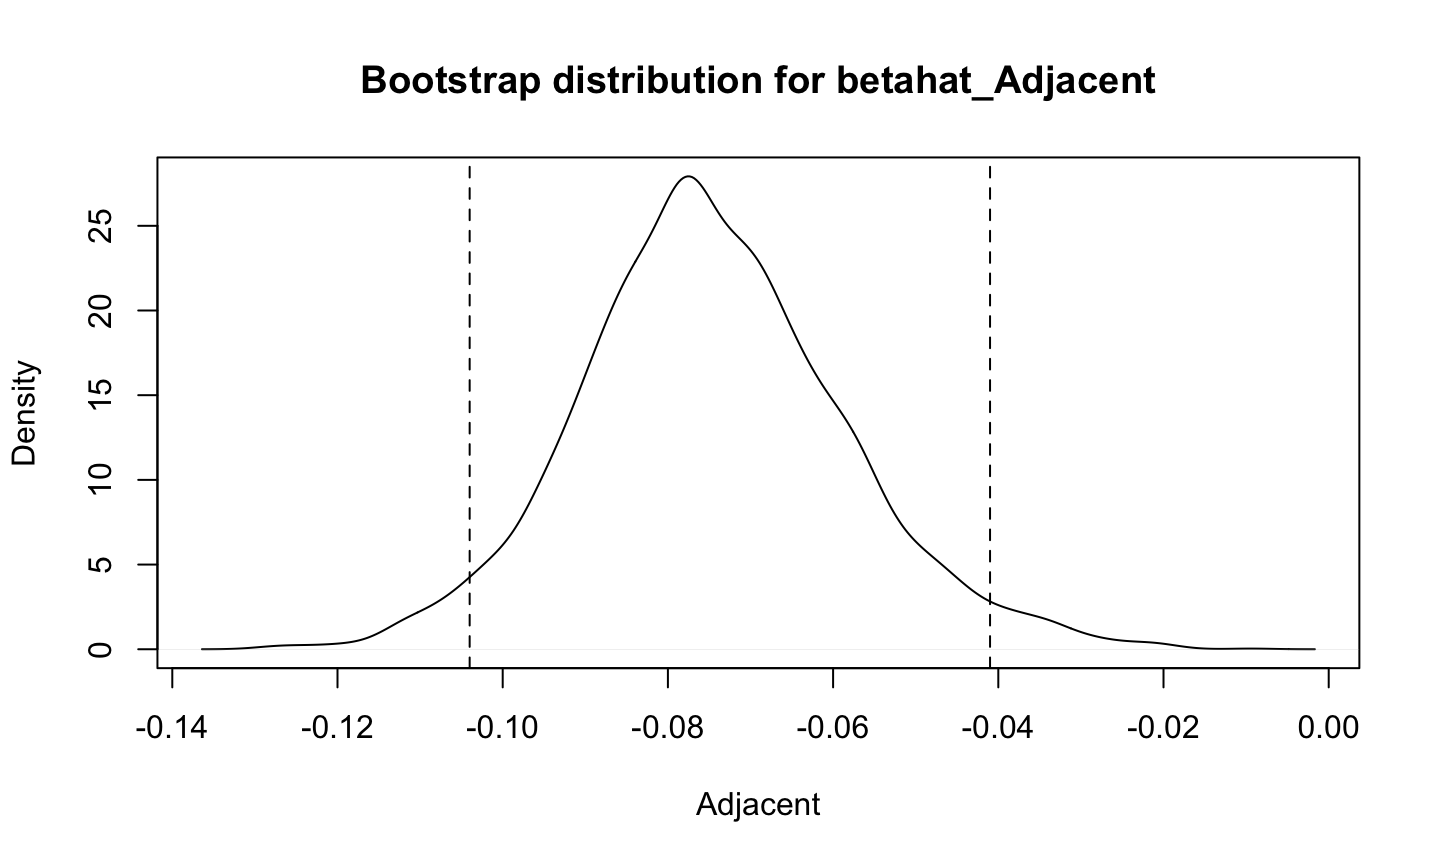
\includegraphics{chapter1_files/figure-beamer/unnamed-chunk-34-1.pdf}

\end{frame}

\begin{frame}[fragile]{What we can tell from the histogram}
\protect\hypertarget{what-we-can-tell-from-the-histogram}{}

The histogram is approximately bell-shaped and centered around 70.

\begin{Shaded}
\begin{Highlighting}[]
\KeywordTok{hist}\NormalTok{(pima}\OperatorTok{$}\NormalTok{dias,}\DataTypeTok{xlab=}\StringTok{"Diastolic"}\NormalTok{,}\DataTypeTok{main=}\StringTok{""}\NormalTok{, }\DataTypeTok{breaks =} \DecValTok{20}\NormalTok{)}
\end{Highlighting}
\end{Shaded}

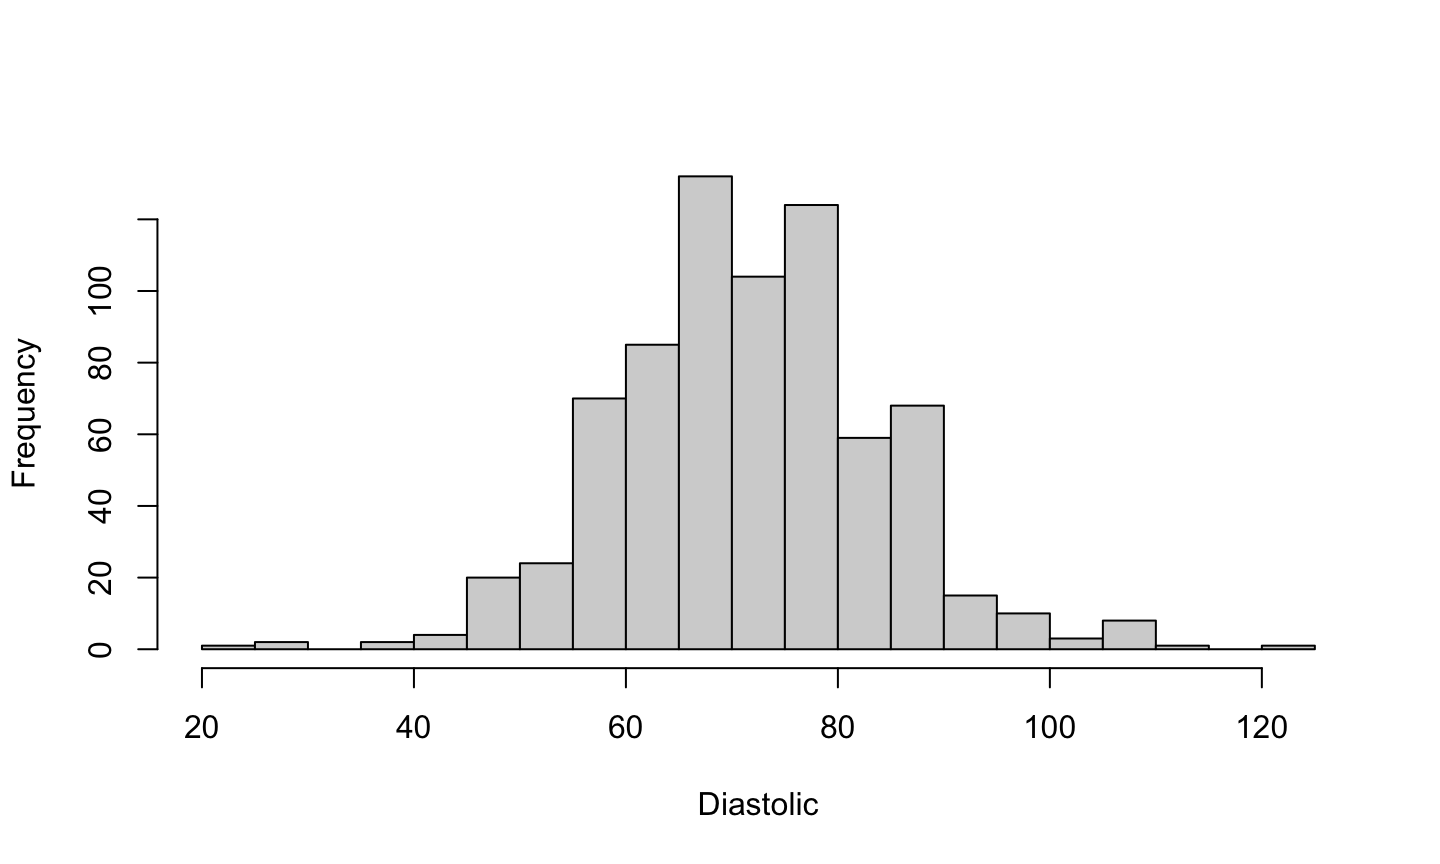
\includegraphics{chapter1_files/figure-beamer/unnamed-chunk-35-1.pdf}

\end{frame}

\begin{frame}{Density plot}
\protect\hypertarget{density-plot}{}

Many people prefer the density plot over the histogram since the
histogram is so sensitive to its options.

\begin{itemize}
\tightlist
\item
  A density plot is essentially a smoothed version of a histogram.
\item
  A ``kernel'' smoother is used to construct a weighted average of data
  points and create a smooth surface.
\end{itemize}

\end{frame}

\begin{frame}[fragile]{Density Plot}
\protect\hypertarget{density-plot-1}{}

The density plot isn't as blocky (though you might see weird things
happen at the boundaries).

\begin{Shaded}
\begin{Highlighting}[]
\KeywordTok{plot}\NormalTok{(}\KeywordTok{density}\NormalTok{(pima}\OperatorTok{$}\NormalTok{diastolic,}\DataTypeTok{na.rm=}\OtherTok{TRUE}\NormalTok{),}\DataTypeTok{main=}\StringTok{""}\NormalTok{)}
\end{Highlighting}
\end{Shaded}

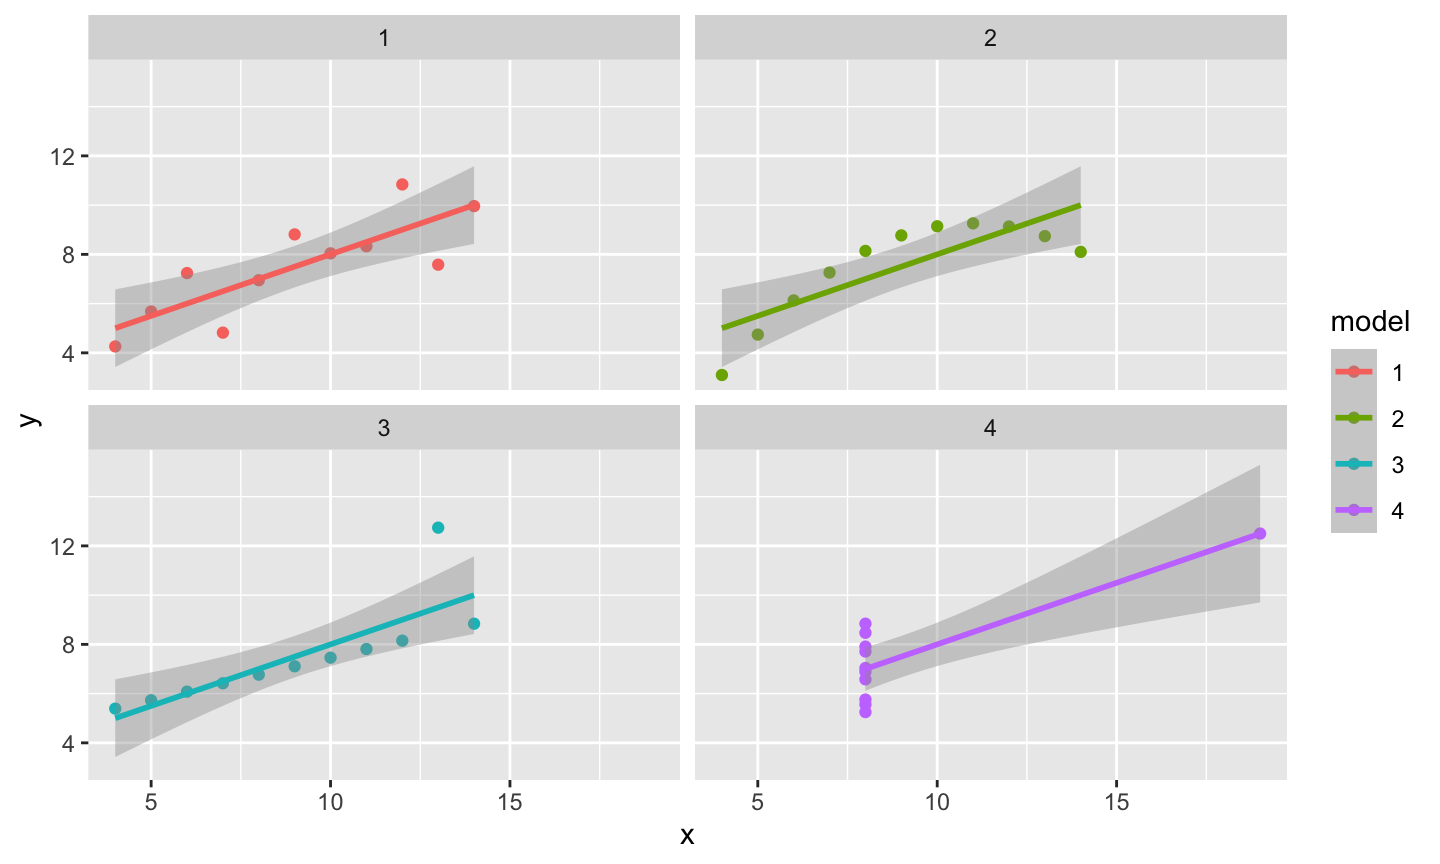
\includegraphics{chapter1_files/figure-beamer/unnamed-chunk-36-1.pdf}

\end{frame}

\begin{frame}[fragile]{Plot points}
\protect\hypertarget{plot-points}{}

We could simply plot the sorted data against its index.

\begin{Shaded}
\begin{Highlighting}[]
\KeywordTok{plot}\NormalTok{(}\KeywordTok{sort}\NormalTok{(pima}\OperatorTok{$}\NormalTok{diastolic),}\DataTypeTok{ylab=}\StringTok{"Sorted Diastolic"}\NormalTok{)}
\end{Highlighting}
\end{Shaded}

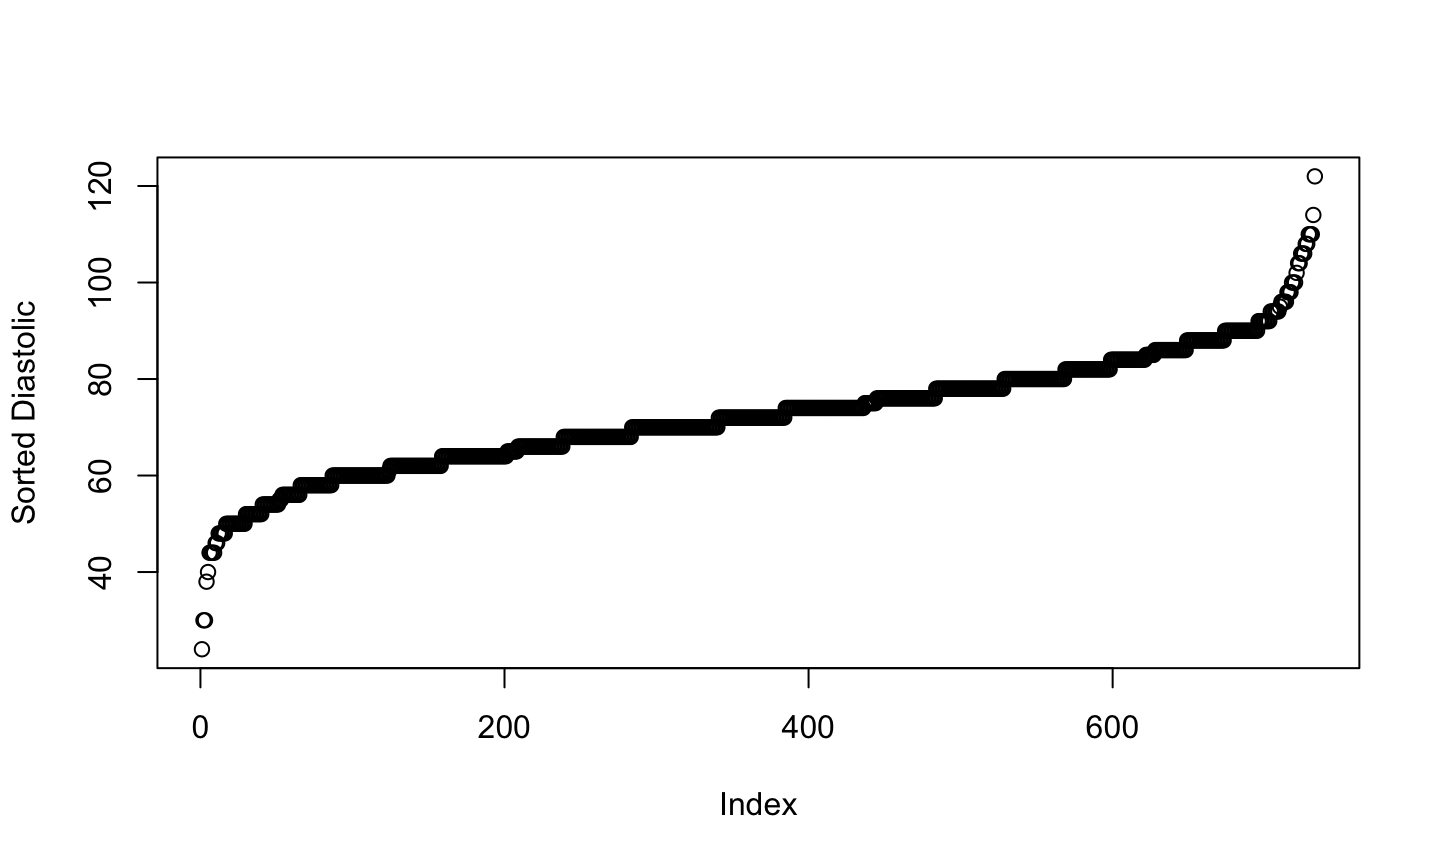
\includegraphics{chapter1_files/figure-beamer/unnamed-chunk-37-1.pdf}

\end{frame}

\begin{frame}{What we see}
\protect\hypertarget{what-we-see}{}

This plot is most useful for identifying:

\begin{itemize}
\tightlist
\item
  Possible outliers
\item
  The discreteness of the data

  \begin{itemize}
  \tightlist
  \item
    Are there numerous repeated data values or are they all unique?
    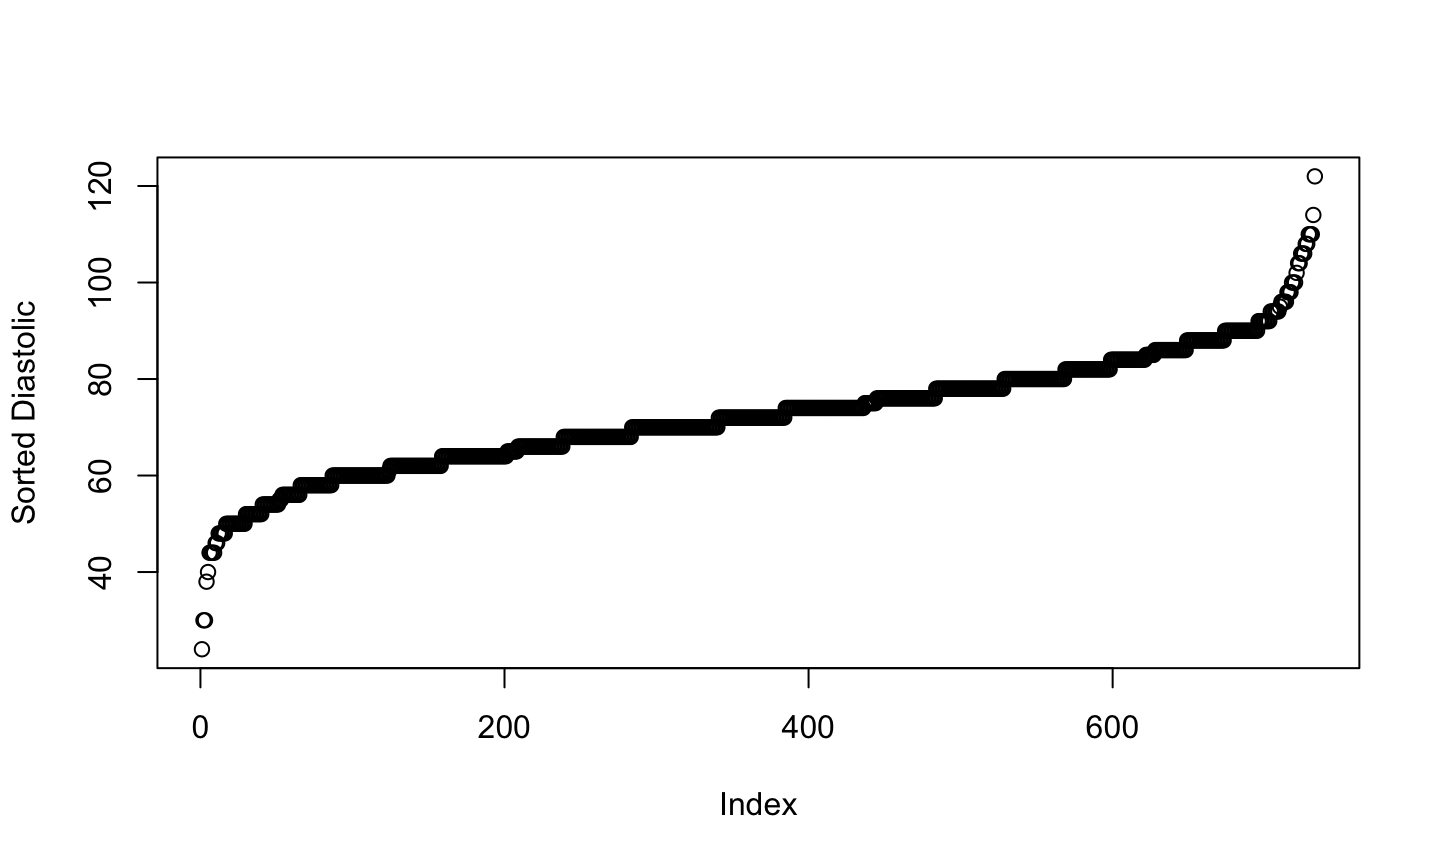
\includegraphics{chapter1_files/figure-beamer/unnamed-chunk-38-1.pdf}
  \end{itemize}
\end{itemize}

\end{frame}

\begin{frame}[fragile]{Bivariate plot}
\protect\hypertarget{bivariate-plot}{}

A standard scatterplot of diabetes vs diastolic blood pressure.

\begin{Shaded}
\begin{Highlighting}[]
\KeywordTok{plot}\NormalTok{(diabetes }\OperatorTok{~}\StringTok{ }\NormalTok{diastolic, }\DataTypeTok{data =}\NormalTok{ pima)}
\end{Highlighting}
\end{Shaded}

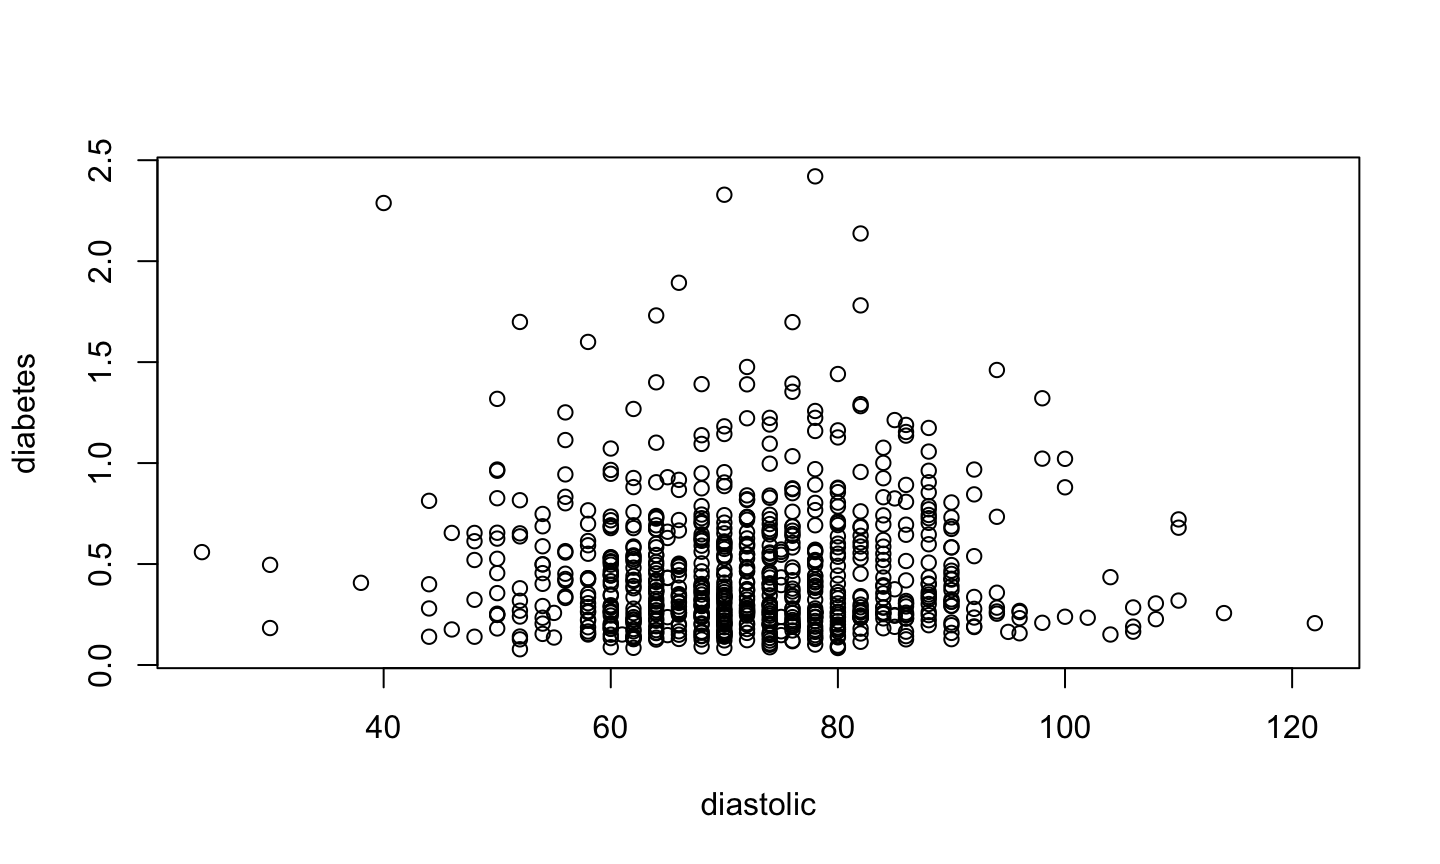
\includegraphics{chapter1_files/figure-beamer/unnamed-chunk-39-1.pdf}

\end{frame}

\begin{frame}[fragile]{Bivariate plot}
\protect\hypertarget{bivariate-plot-1}{}

A parallel boxplot of diabetes vs test result.

\begin{Shaded}
\begin{Highlighting}[]
\KeywordTok{plot}\NormalTok{(diabetes }\OperatorTok{~}\StringTok{ }\NormalTok{test, }\DataTypeTok{data =}\NormalTok{ pima)}
\end{Highlighting}
\end{Shaded}

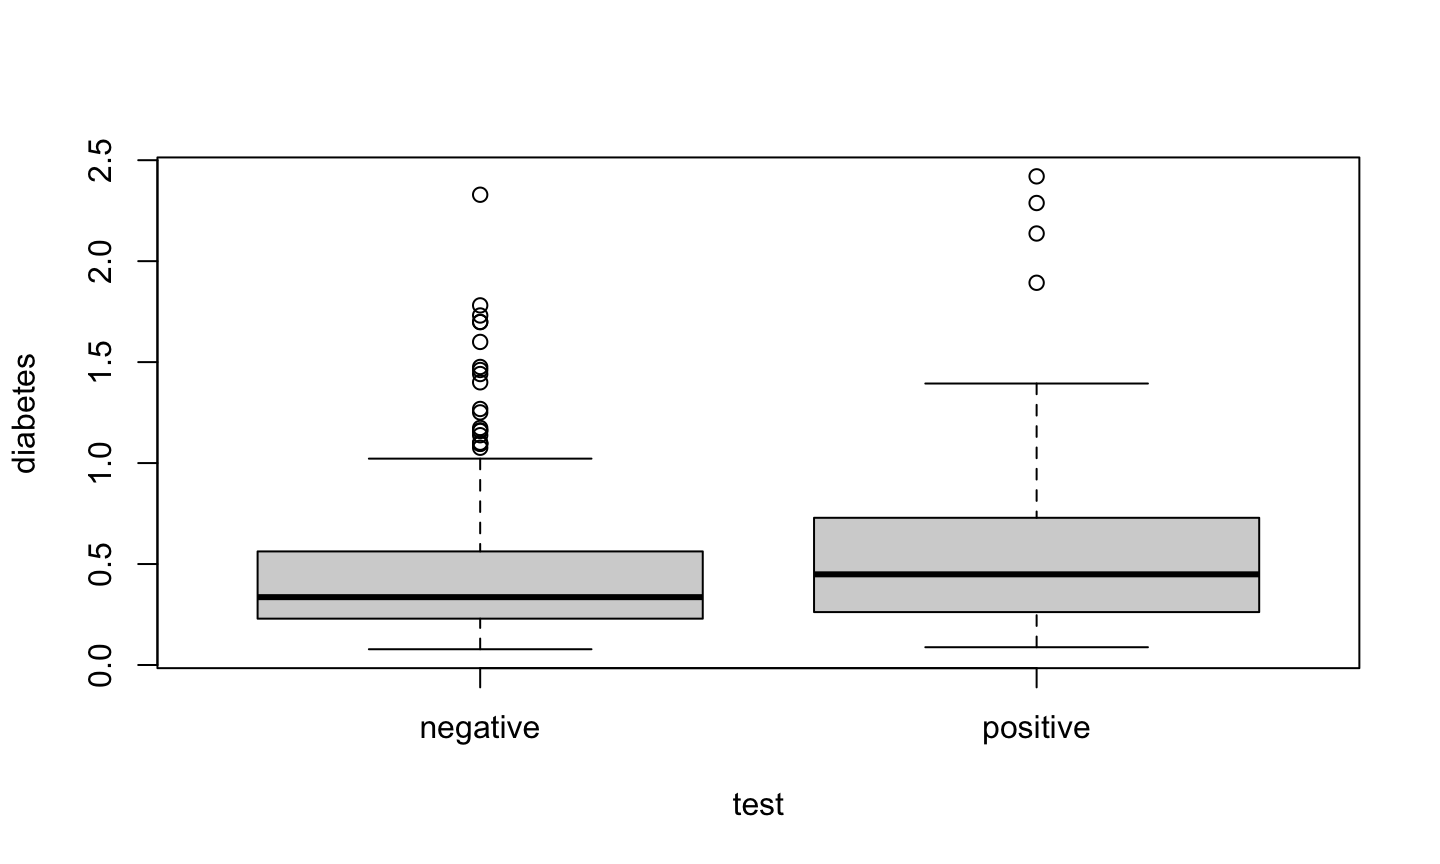
\includegraphics{chapter1_files/figure-beamer/unnamed-chunk-40-1.pdf}

\end{frame}

\begin{frame}[fragile]{Side by side plots}
\protect\hypertarget{side-by-side-plots}{}

\begin{Shaded}
\begin{Highlighting}[]
\KeywordTok{par}\NormalTok{(}\DataTypeTok{mfrow=}\KeywordTok{c}\NormalTok{(}\DecValTok{1}\NormalTok{,}\DecValTok{2}\NormalTok{))}
\KeywordTok{plot}\NormalTok{(diabetes }\OperatorTok{~}\StringTok{ }\NormalTok{diastolic, }\DataTypeTok{data =}\NormalTok{ pima)}
\KeywordTok{plot}\NormalTok{(diabetes }\OperatorTok{~}\StringTok{ }\NormalTok{test, }\DataTypeTok{data =}\NormalTok{ pima)}
\end{Highlighting}
\end{Shaded}

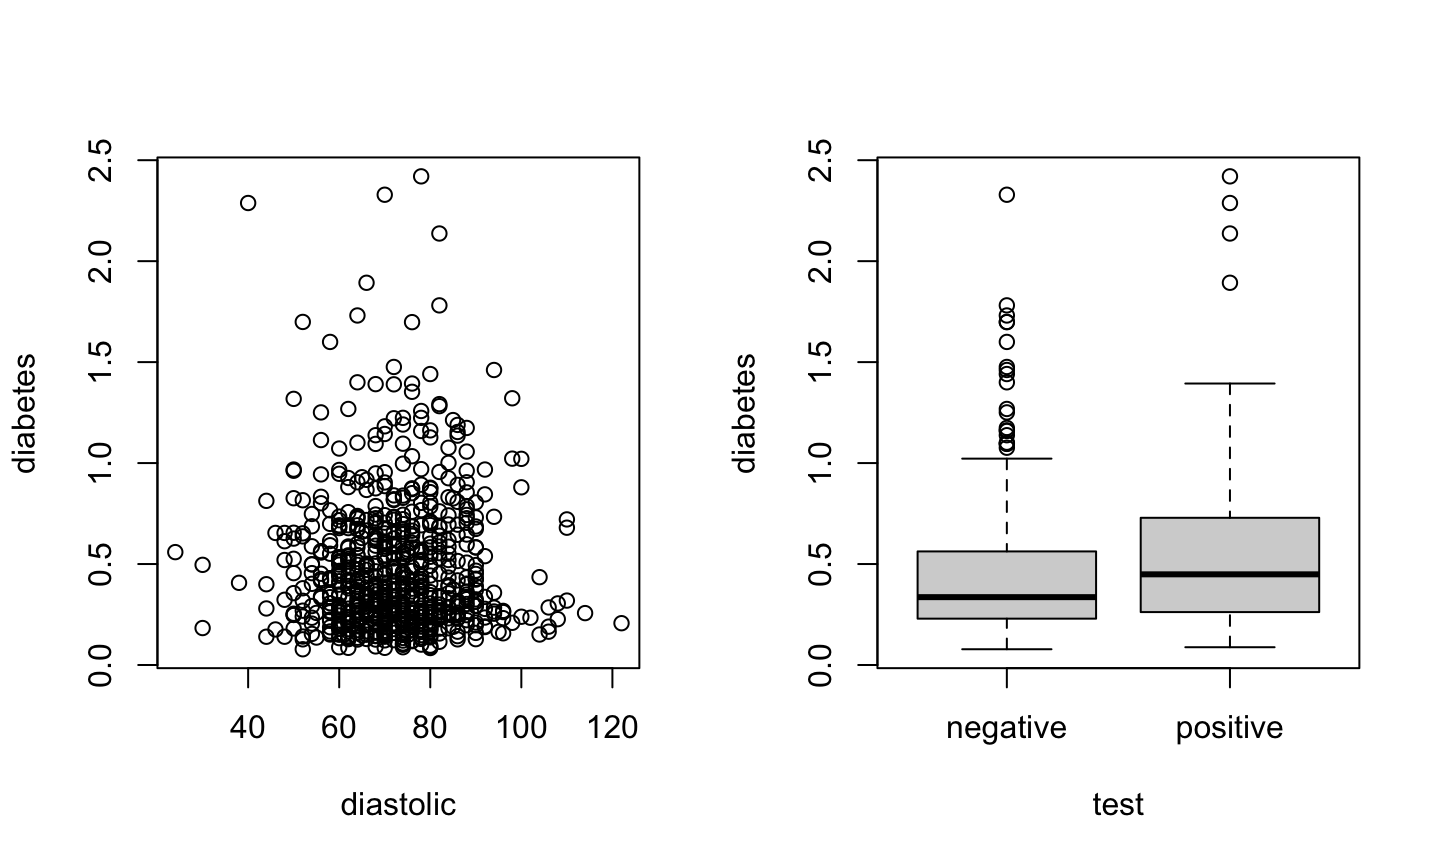
\includegraphics{chapter1_files/figure-beamer/unnamed-chunk-41-1.pdf}

\end{frame}

\begin{frame}[fragile]{\texttt{ggplot2}}
\protect\hypertarget{ggplot2}{}

The plots we have just created are using the base graphics system in R.
- These are very fast, simple, and professional.

A fancier alternative is to construct plots using the \texttt{ggplot2}
package.

In its simplest form, \texttt{ggplot2} requires you to provide:

\begin{itemize}
\tightlist
\item
  A ggplot object that includes the data frame holding the data.
\item
  A mapping arguments that specifies the plot aesthetics (essentially,
  the data that will be used in the plot).
\item
  A geometry object that specifies how the aesthetics are used in a
  plot.
\end{itemize}

\end{frame}

\begin{frame}[fragile]{\texttt{ggplot2} example}
\protect\hypertarget{ggplot2-example}{}

\begin{Shaded}
\begin{Highlighting}[]
\KeywordTok{library}\NormalTok{(ggplot2)}
\NormalTok{ggpima  =}\StringTok{ }\KeywordTok{ggplot}\NormalTok{(pima, }\KeywordTok{aes}\NormalTok{(}\DataTypeTok{x=}\NormalTok{diastolic))}
\NormalTok{ggpima }\OperatorTok{+}\StringTok{ }\KeywordTok{geom_histogram}\NormalTok{(}\KeywordTok{aes}\NormalTok{(}\DataTypeTok{x =}\NormalTok{ diastolic))}
\end{Highlighting}
\end{Shaded}

\begin{verbatim}
## `stat_bin()` using `bins = 30`. Pick better value with `binwidth`.
\end{verbatim}

\begin{verbatim}
## Warning: Removed 35 rows containing non-finite values (stat_bin).
\end{verbatim}

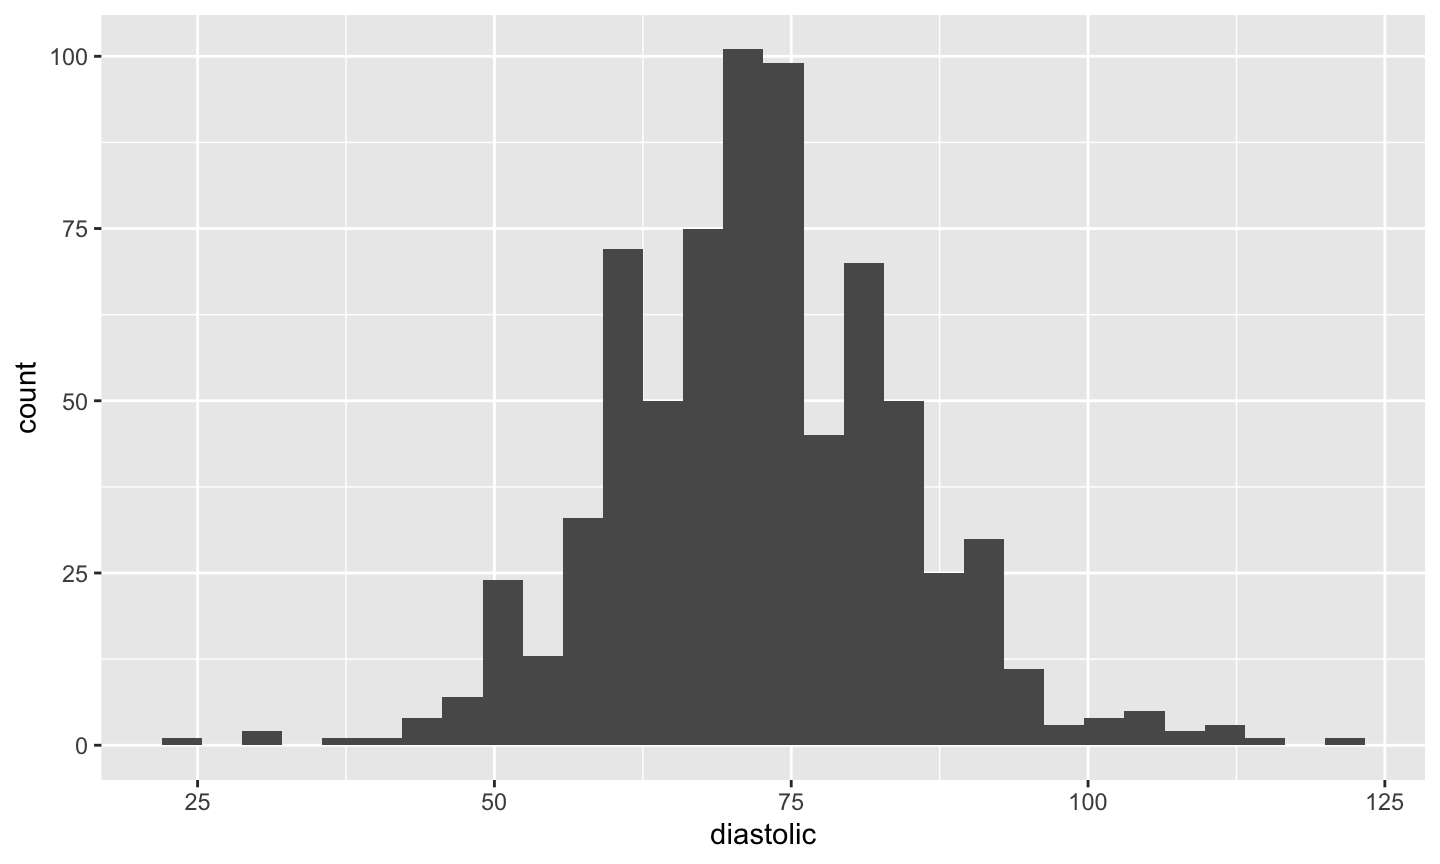
\includegraphics{chapter1_files/figure-beamer/unnamed-chunk-42-1.pdf}

\end{frame}

\begin{frame}[fragile]{\texttt{ggplot2} example}
\protect\hypertarget{ggplot2-example-1}{}

\begin{Shaded}
\begin{Highlighting}[]
\NormalTok{ggpima }\OperatorTok{+}\StringTok{ }\KeywordTok{geom_density}\NormalTok{(}\KeywordTok{aes}\NormalTok{(}\DataTypeTok{x =}\NormalTok{ diastolic))}
\end{Highlighting}
\end{Shaded}

\begin{verbatim}
## Warning: Removed 35 rows containing non-finite values (stat_density).
\end{verbatim}

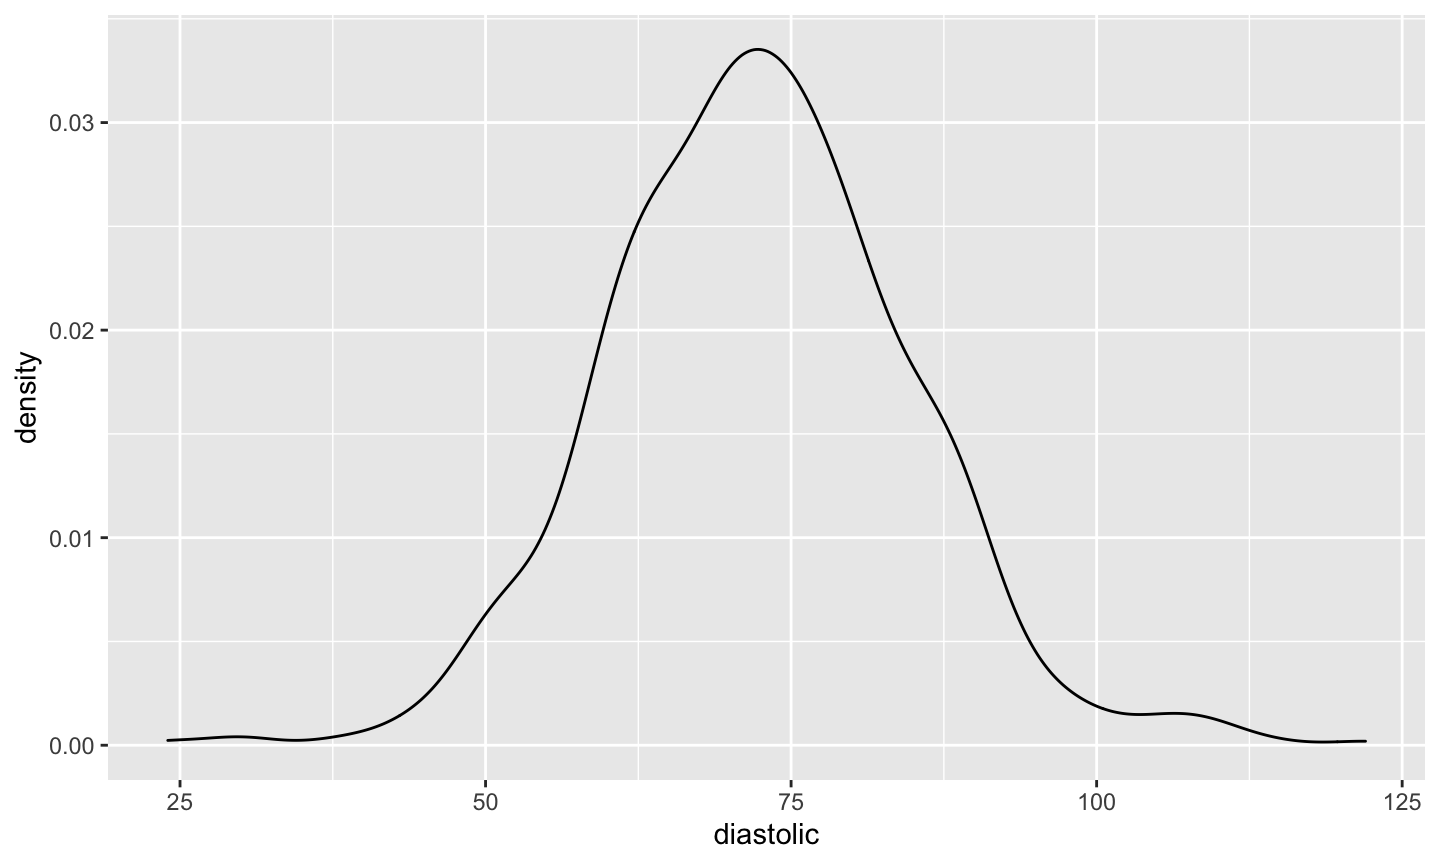
\includegraphics{chapter1_files/figure-beamer/unnamed-chunk-43-1.pdf}

\end{frame}

\begin{frame}[fragile]{\texttt{ggplot2} example}
\protect\hypertarget{ggplot2-example-2}{}

\begin{Shaded}
\begin{Highlighting}[]
\NormalTok{ggpima }\OperatorTok{+}\StringTok{ }\KeywordTok{geom_point}\NormalTok{(}\KeywordTok{aes}\NormalTok{(}\DataTypeTok{x =}\NormalTok{ diastolic, }\DataTypeTok{y =}\NormalTok{ diabetes))}
\end{Highlighting}
\end{Shaded}

\begin{verbatim}
## Warning: Removed 35 rows containing missing values (geom_point).
\end{verbatim}

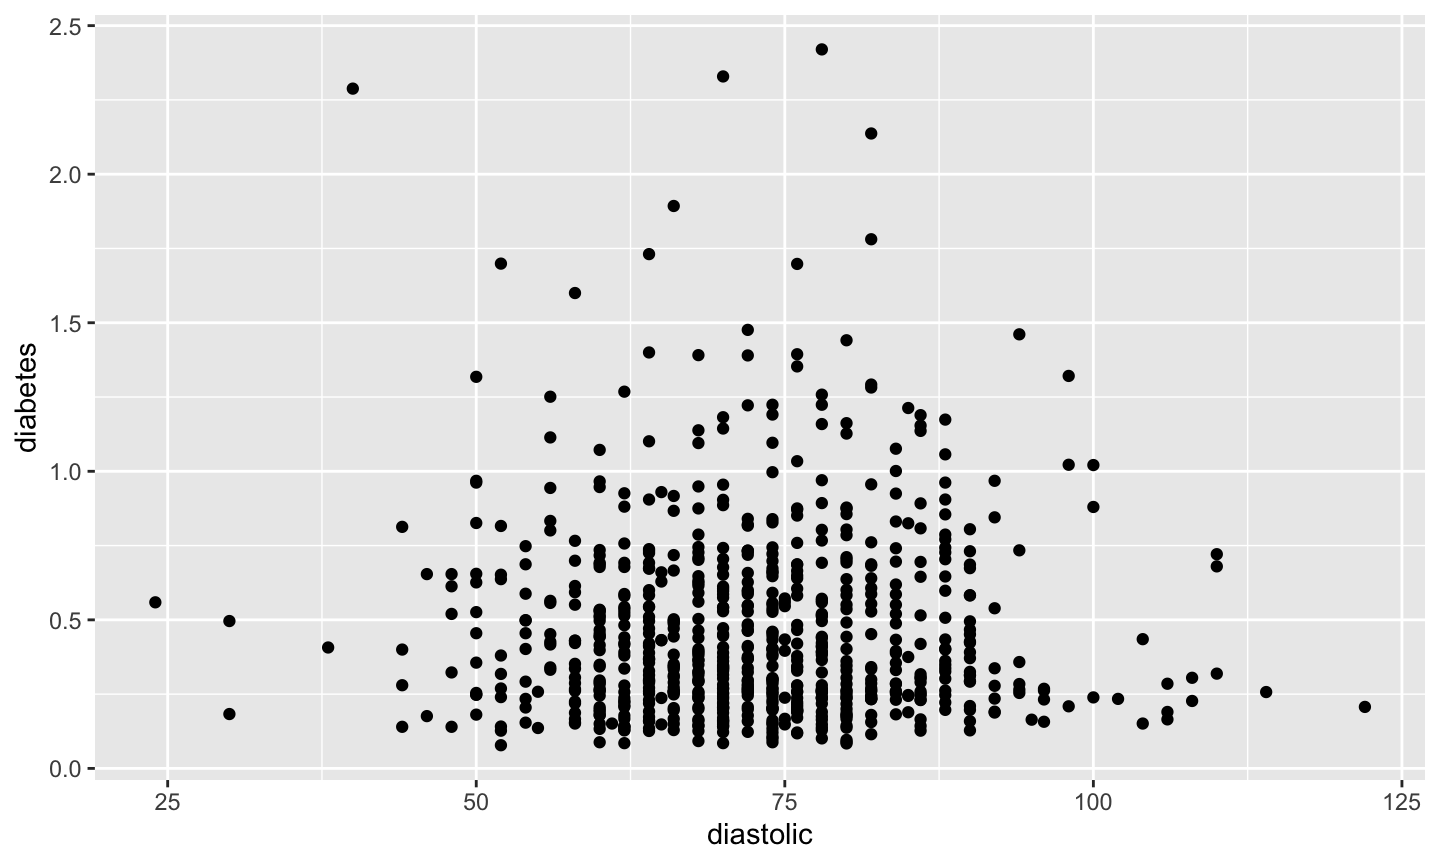
\includegraphics{chapter1_files/figure-beamer/unnamed-chunk-44-1.pdf}

\end{frame}

\begin{frame}[fragile]{Customize \texttt{ggplot2}}
\protect\hypertarget{customize-ggplot2}{}

\begin{Shaded}
\begin{Highlighting}[]
\NormalTok{ggpima }\OperatorTok{+}\StringTok{ }
\StringTok{  }\KeywordTok{geom_point}\NormalTok{(}\KeywordTok{aes}\NormalTok{(}\DataTypeTok{x =}\NormalTok{ diastolic, }\DataTypeTok{y =}\NormalTok{ diabetes, }\DataTypeTok{shape =}\NormalTok{ test)) }\OperatorTok{+}\StringTok{ }
\StringTok{  }\KeywordTok{theme}\NormalTok{(}\DataTypeTok{legend.position =} \StringTok{"top"}\NormalTok{, }\DataTypeTok{legend.direction =} \StringTok{"horizontal"}\NormalTok{)}
\end{Highlighting}
\end{Shaded}

\begin{verbatim}
## Warning: Removed 35 rows containing missing values (geom_point).
\end{verbatim}

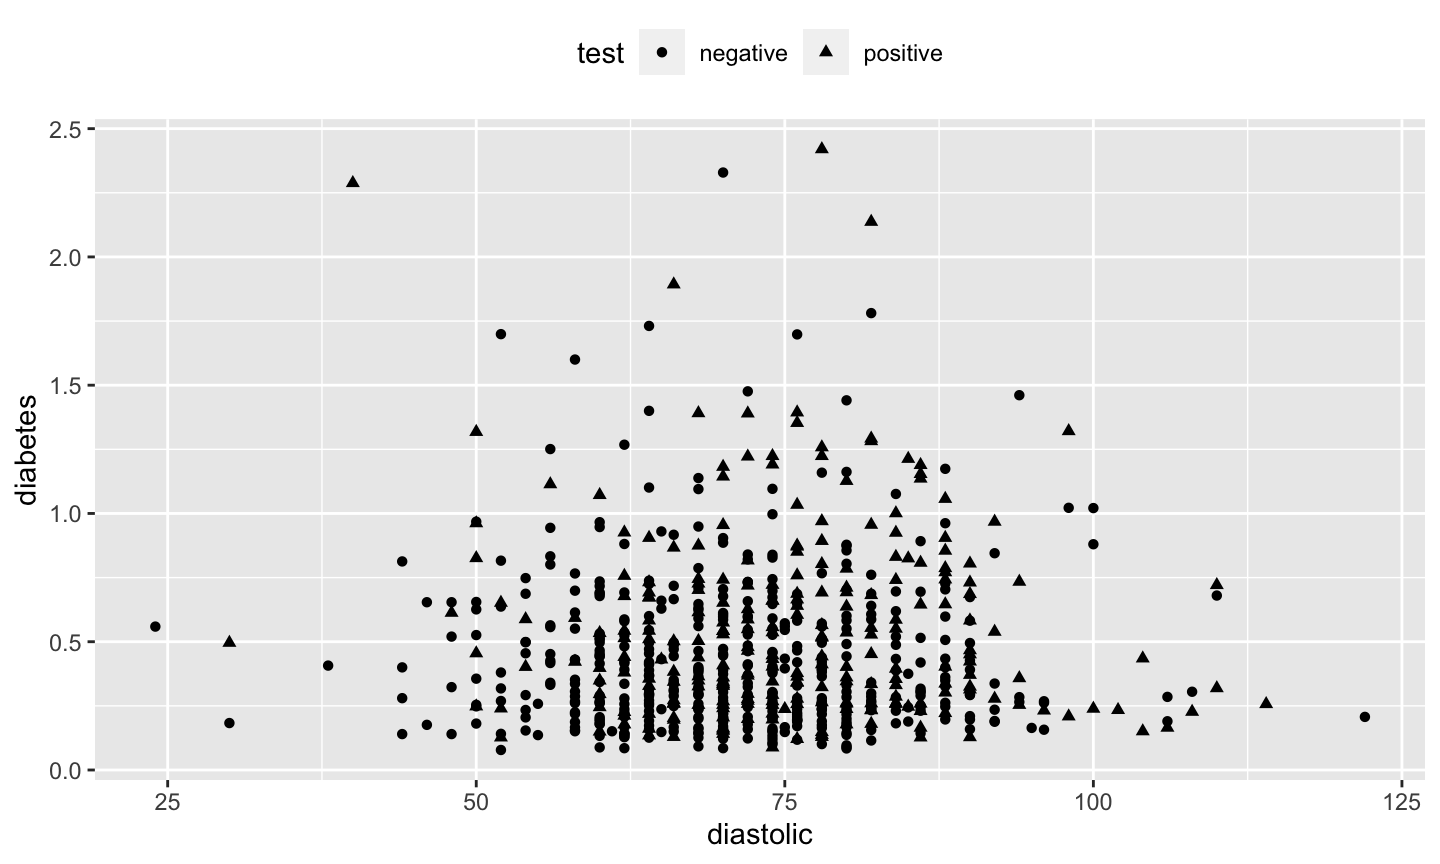
\includegraphics{chapter1_files/figure-beamer/unnamed-chunk-45-1.pdf}

\end{frame}

\begin{frame}[fragile]{Faceting \texttt{ggplot2}}
\protect\hypertarget{faceting-ggplot2}{}

\begin{verbatim}
## Warning: Removed 35 rows containing missing values (geom_point).
\end{verbatim}

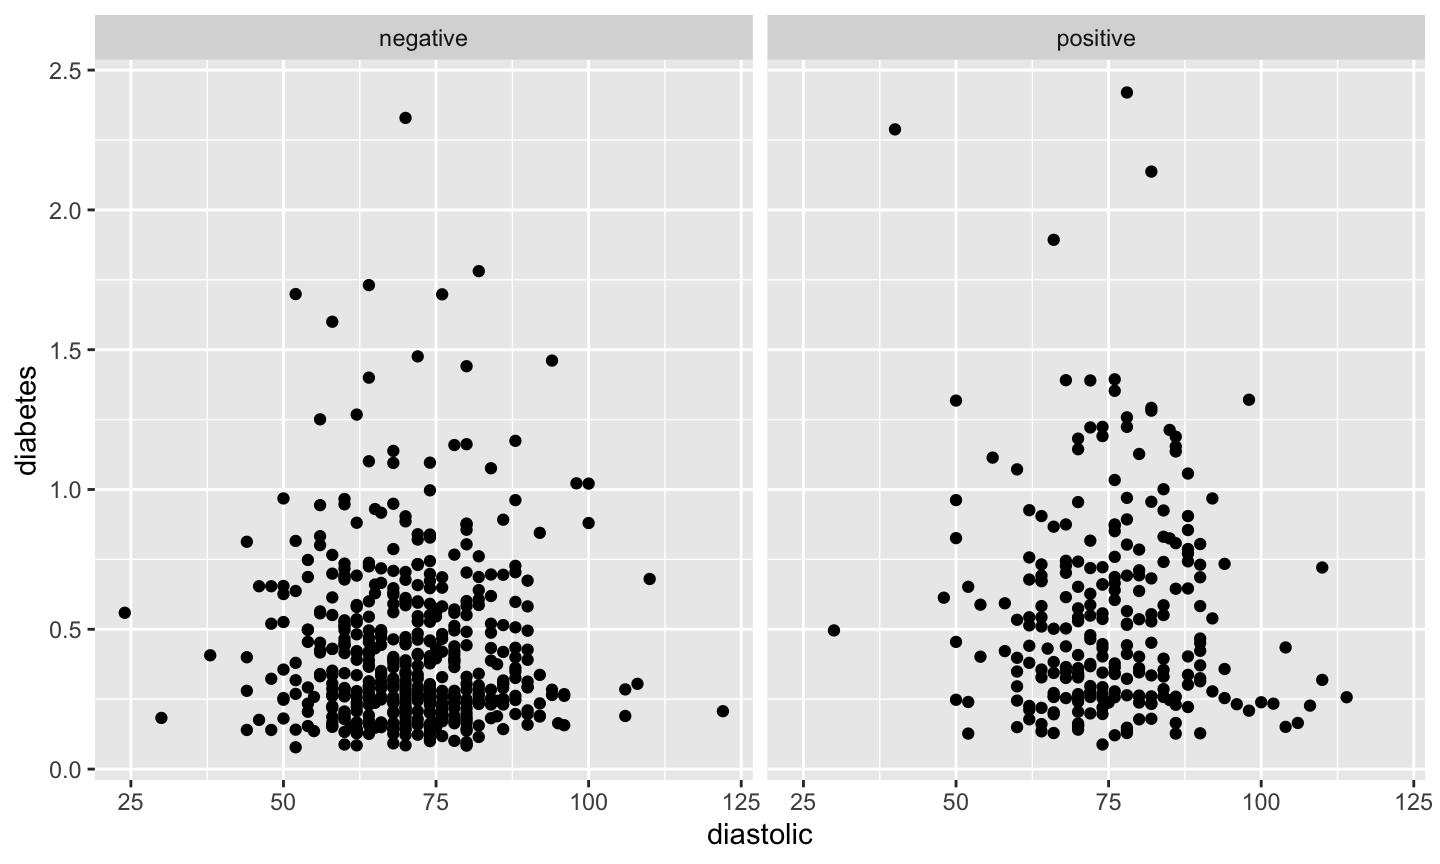
\includegraphics{chapter1_files/figure-beamer/unnamed-chunk-46-1.pdf}

\end{frame}

\begin{frame}[fragile]{Summary of \texttt{ggplot2}}
\protect\hypertarget{summary-of-ggplot2}{}

\begin{itemize}
\tightlist
\item
  You first need to create a ggplot object using the \texttt{ggplot}
  function. Specify: o- The data frame the data is contained in (e.g.,
  the data frame is \texttt{pima})
\item
  Map the \textbf{aesthetics} using \texttt{aes}. The aesthetic
  specifies what you see, such as position in the \(x\) or \(y\)
  direction or aspects such as shape or color.
\item
  Specify the geometry for the plot (how you want to map the
  aesthetics).
\item
  The advantage of \texttt{ggplot2} is more apparent in producing more
  complex plots involving more than just two variables.
\item
  A \texttt{theme} specifies options for the appearance of the plot.
\item
  We specified where the \texttt{legend} should appear in one plot and
  to use more than one panel (\texttt{facets}) in another.
\end{itemize}

\end{frame}

\hypertarget{when-to-use-linear-modeling}{%
\section{When to Use Linear
Modeling}\label{when-to-use-linear-modeling}}

\begin{frame}{Linear Models}
\protect\hypertarget{linear-models}{}

Linear models are used to model the relationship between a:

\begin{itemize}
\tightlist
\item
  single variable \(Y\), called the \textbf{response, outcome, output,
  or dependent} variable and
\item
  one or more \textbf{predictor, input, independent, or explanatory}
  variables.
\end{itemize}

Note: the descriptions of independent and dependent variables are vague
and are best avoided.

\textbf{Regression analysis} is another term for linear modeling,
although regressions can be nonlinear.

\end{frame}

\begin{frame}{Terminology and Assumptions}
\protect\hypertarget{terminology-and-assumptions}{}

\begin{itemize}
\tightlist
\item
  When we have one constant predictor and one non-constant predictor, we
  are doing simple regression.\\
\item
  When we have more than one non-constant predictor we are doing
  multiple regression.
\item
  When we have more than one response, we are doing multivariate
  regression.
\end{itemize}

Assumptions of linear models: - Y is (approximately) continuous -
Predictors can be continuous, discrete, or categorical.

\end{frame}

\begin{frame}{More terminology}
\protect\hypertarget{more-terminology}{}

\begin{itemize}
\tightlist
\item
  A regression with one quantitative predictor and one qualitative
  predictor is an \textbf{analysis of covariance (ANCOVA)}.
\item
  A regression with all qualitative predictors is an \textbf{analysis of
  variance (ANOVA)}.
\item
  A regression with a qualitative response will typically utilize
  \textbf{logistic} regression.
\item
  Responses that do not have a normal distribution are modeled using
  \textbf{generalized linear models (GLMs)}.
\end{itemize}

\end{frame}

\begin{frame}{Goals of regression}
\protect\hypertarget{goals-of-regression}{}

\begin{enumerate}
\tightlist
\item
  Prediction of future or unseen responses given specified values of the
  predictors.
\item
  Assessments of the effect of, or relationship between, explanatory
  variables and the response. We would like to infer causal
  relationships if possible.
\end{enumerate}

Be clear of your objective! Your choice of analysis may differ depending
on the objective.

There is generally no \textbf{true} model. We simply want to find a
model that adequately describes the relationship between relevant
explanatory variables, allows us to make good predictions, infer
causality, etc.

\end{frame}

\hypertarget{more-discussion-on-scatterplots}{%
\section{More discussion on
scatterplots}\label{more-discussion-on-scatterplots}}

\begin{frame}{Height example}
\protect\hypertarget{height-example}{}

Scatterplots are a convenient way to study the dependence between a
single response and a single predictor variable.

\textbf{Inheritance of Height}

Karl Pearson (1857-1936) organized the collection of n=1375 heights of
mothers in the United Kingdom under the age of 65 and one of their adult
daughters over the age of 18. We are interested in the inheritance from
the mother to the daughter, so the mother's height (mheight) is used as
the predictor variable and the daughter's height (dheight) is used as
the response variable.

\end{frame}

\begin{frame}{Heritability}
\protect\hypertarget{heritability}{}

Do taller mothers tend to have taller daughters? Do shorter mothers tend
to have shorter daughters?

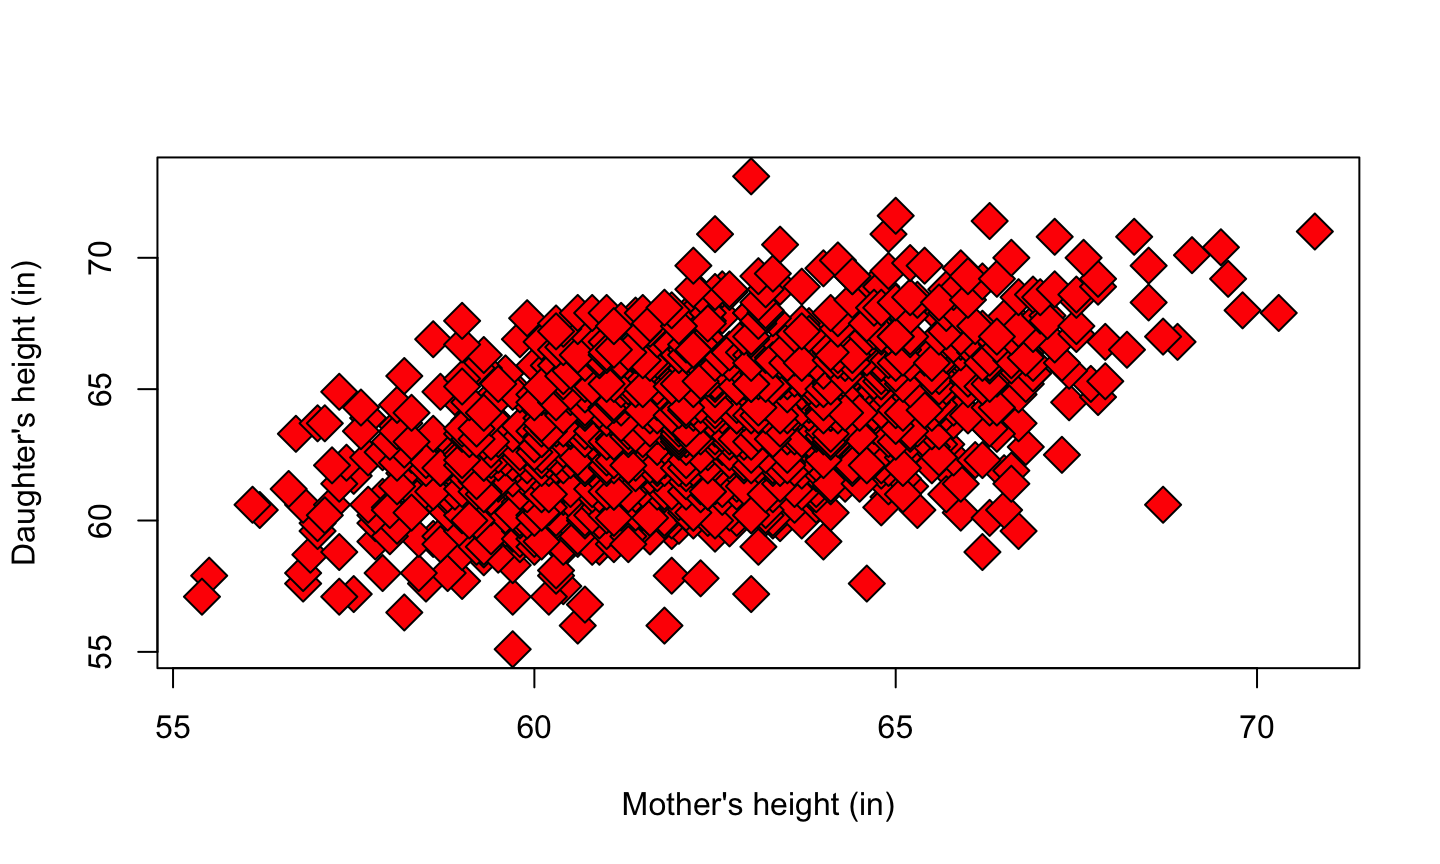
\includegraphics{chapter1_files/figure-beamer/unnamed-chunk-47-1.pdf}

\end{frame}

\begin{frame}{What the plot says}
\protect\hypertarget{what-the-plot-says}{}

\begin{itemize}
\item
  Notice that since the range of the measurements are roughly the same
  for the two variables, we use the same scale for the x and y-axis.
\item
  There is a clear linear relationship between the heights of mothers
  and daughters.
\item
  Notice that there are more points in the center of the data, and fewer
  points along the edges. This is typical for biological data.
\end{itemize}

\end{frame}

\begin{frame}[fragile]{Car data}
\protect\hypertarget{car-data}{}

The data give the speed of cars and the distances taken to stop. Note
that the data were recorded in the 1920s.

\begin{verbatim}
## [1] "speed" "dist"
\end{verbatim}

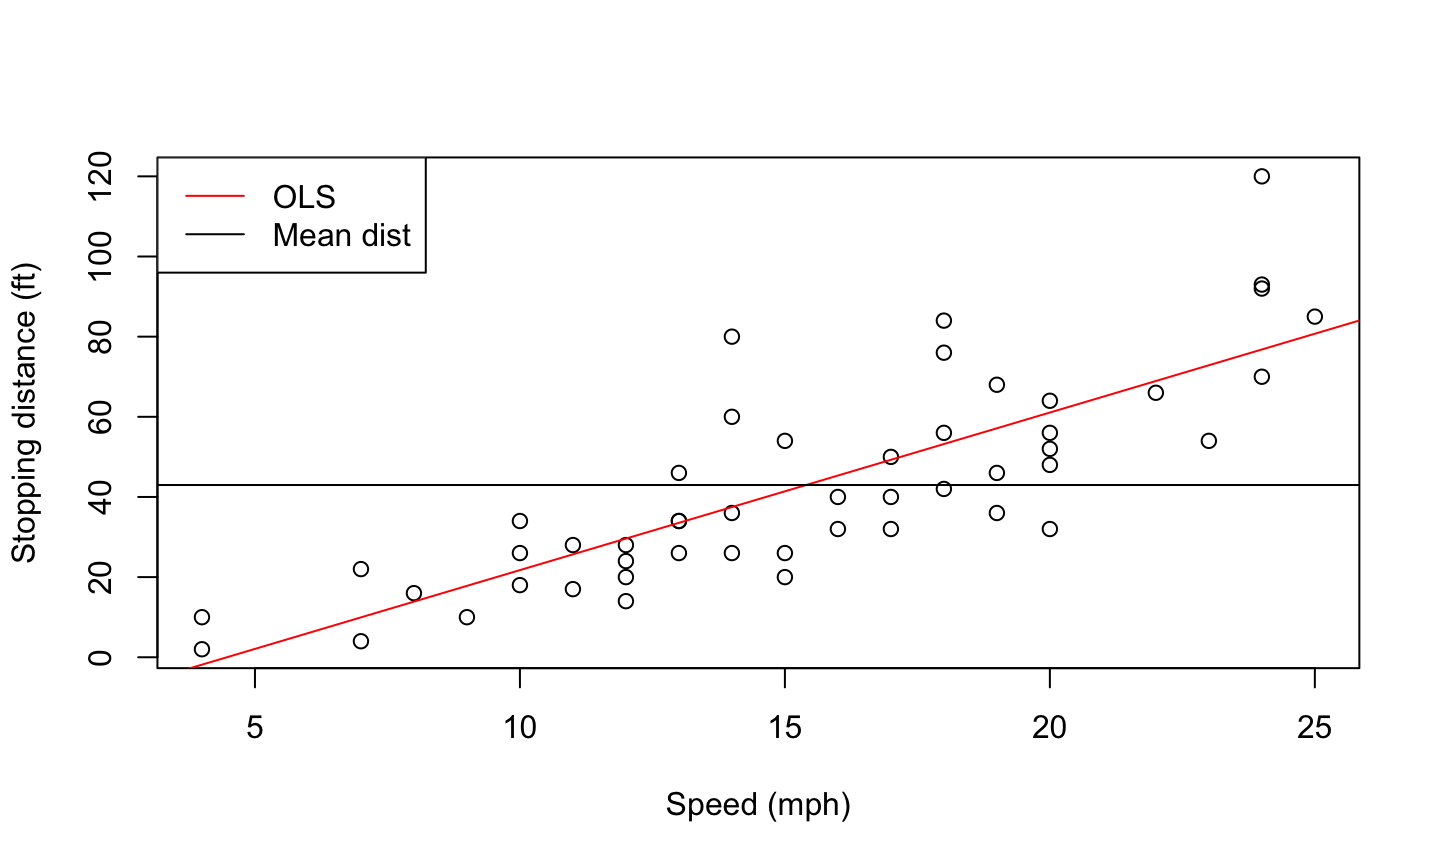
\includegraphics{chapter1_files/figure-beamer/unnamed-chunk-48-1.pdf}

\end{frame}

\hypertarget{mean-functions}{%
\section{Mean Functions}\label{mean-functions}}

\begin{frame}{Mean Function}
\protect\hypertarget{mean-function}{}

We are frequently interested in how the distribution of the response
varies with changes in the predictor variable.

The \textbf{mean function} is particularly important, and we define it
by the relationship

\(E(Y│X=x)=a\) function the depends on the value of x.

We read this as the ``expected value of the response when the predictor
is fixed at the value \(X=x\)''

\end{frame}

\begin{frame}{Mean Function}
\protect\hypertarget{mean-function-1}{}

For example, in the Heights data, we might believe that

\(E(dheight│mheight=x)=β_0+β_1 x\),

that is, the mean function is a straight line.

The particular mean function has two parameters, an intercept
\(\beta_0\) and a slope \(\beta_1\).

If we knew the values of the \(\beta\)s, then the mean function would be
completely known. In practice, these must be estimated from the data.

If the response variable and the predictor variable are independent
(have no relationship), then \(\beta_1=0\). We will learn how to test
this hypothesis later.

\end{frame}
